\documentclass[conference,twocolumn,a4paper]{IEEEtran}

\usepackage{amsmath,amssymb,bm}
\usepackage{cite}
\usepackage{fontspec}
\usepackage{graphicx}
\usepackage{tikz}
\usepackage{subcaption}
\usepackage{stfloats}
\usepackage{cuted}
\usepackage{placeins}
\usepackage{booktabs}
\usepackage{multirow}
\usepackage{algorithm}
\usepackage{algpseudocode}
\usepackage{url}
\usepackage{xeCJK}

\graphicspath{{figure/}{AN_simulation/}}

\setlength{\textfloatsep}{8pt plus 2pt minus 2pt}
\setlength{\dbltextfloatsep}{8pt plus 2pt minus 2pt}
\setlength{\floatsep}{8pt plus 2pt minus 2pt}
\setlength{\intextsep}{8pt plus 2pt minus 2pt}
\setlength{\abovecaptionskip}{4pt plus 1pt minus 1pt}
\setlength{\belowcaptionskip}{0pt}

\makeatletter
\setlength{\@fptop}{0pt}
\setlength{\@fpsep}{8pt plus 1fil}
\setlength{\@fpbot}{0pt plus 1fil}
\setlength{\@dblfptop}{0pt}
\setlength{\@dblfpsep}{8pt plus 1fil}
\setlength{\@dblfpbot}{0pt plus 1fil}
\makeatother

\setCJKmainfont{FandolSong-Regular}

\DeclareMathOperator*{\argmax}{arg\,max}
\DeclareMathOperator*{\argmin}{arg\,min}
\newcommand{\verifytag}{[待根据原文件进一步核实]}

\title{Artificial-Noise-Aided Secure Sensing in Multi-Static Cell-Free Massive MIMO ISAC With an Internal Adversary}

\author{\IEEEauthorblockN{Author information to be inserted \verifytag}}

\begin{document}

\maketitle

\begin{abstract}
This paper investigates sensing privacy protection in a multi-static cell-free massive MIMO integrated sensing and communication system, focusing on the threat that an internal legitimate user steals target-location information through signal reconstruction. Such an adversary does not need to crack the communication protocol. Instead, it passively intercepts the received signal, estimates the components not transmitted by itself via the EM algorithm, and further reconstructs the beampatterns of the transmitting APs, thereby inferring the true target position from spatial clues. To mitigate this leakage process, this paper proposes an artificial-noise-aided joint beam design method that jointly optimizes communication beams, sensing beams, and deceptive artificial-noise beams. The optimization objective is to maximize the legitimate sensing SNR while satisfying user QoS, per-AP power budgets, artificial-noise communication null-space constraints, and fake-direction peak constraints. To solve the resulting non-convex problem, a CCCP-MMSE alternating iterative framework is developed.
 Simulation results show that the proposed method can construct misleading pseudo-peaks while maintaining legitimate sensing performance, 
 substantially lowering its average detection probability while consistently preserving sensing SNR above 32 dB.
\end{abstract}

\begin{IEEEkeywords}
cell-free massive MIMO, integrated sensing and communication, sensing privacy, artificial noise, internal adversary, multi-static sensing.
\end{IEEEkeywords}

\section{Introduction}
Integrated sensing and communication (ISAC) is widely regarded as an important 6G candidate because it can accomplish data transmission and environmental sensing within a unified spectrum, hardware, and waveform framework \cite{wei2022multifunctional}. Smart-city, industrial automation, and intelligent-transportation scenarios further strengthen this demand because the network is expected to support communication and sensing simultaneously under limited resources. The idea of ISAC did not emerge only recently, since early studies had already discussed the possibility of embedding communication information into radar signals \cite{mealey1963}. Subsequent multifunctional communication-radar architectures and sequence-based integrated radar-communication designs reflected the idea of using radar waveforms as carriers for communication signaling \cite{saddik2007,jamil2008}. Recent studies have further shifted the focus to joint spatial design, where communication and sensing beams are generated within a unified optimization framework \cite{liu2020joint}. Estimation-oriented designs also show that sensing-accuracy metrics can be embedded directly into the joint ISAC optimization model, thereby substantially improving target estimation accuracy \cite{liu2022crb}.

Cell-free massive MIMO provides a natural network architecture for this direction because a central processor can coordinate many distributed APs, thereby removing rigid cell boundaries and creating a larger virtual array aperture \cite{ngo2017cellfree}. This distributed structure is especially attractive for ISAC. On the one hand, the enlarged effective aperture improves sensing accuracy and significantly reduces the deployment cost of a dedicated sensing network. On the other hand, sensing-acquired location and velocity information can be reused in communication modules such as channel estimation to improve transmission efficiency. Existing studies have established joint communication-and-sensing beamforming models for cell-free massive MIMO ISAC \cite{demirhan2024cellfreetcom}. Target detection and power allocation in CF-mMIMO-ISAC have also been analyzed \cite{behdad2024multistatic}. Performance analysis further shows that power control is crucial for balancing sensing and communication tasks \cite{nguyen2024multistaticcf}. The communication-sensing-region study in \cite{mao2024region} also compares cell-free and conventional cellular deployment and verifies the radar-sensing advantage of CF-mMIMO.

The other side of this efficiency gain is a sharper security problem. Physical-layer security has long been a fundamental issue in massive MIMO systems because, by virtue of wireless broadcasting, exploitable signal structure is exposed to unauthorized receivers \cite{kapetanovic2015physical}. In this context, artificial noise becomes an important countermeasure because it can directly degrade unauthorized receivers at the signal level \cite{goel2008guaranteeing}. In the ISAC setting, secure radar-communication design in the presence of malicious targets shows that metrics such as the CRLB and secrecy rate are important measures of security performance \cite{art:su2021}. Overall, existing ISAC physical-layer security studies still focus mainly on communication secrecy or external sensing-eavesdropping scenarios, such as suspicious radar receivers, malicious targets, or independent illegal users \cite{chalise2018performance,ren2023robust,zou2024securing}.

This issue becomes more prominent in CF-mMIMO-ISAC. Distributed APs improve communication and sensing performance on the one hand, while also providing potential adversaries with multiple jointly usable spatial observations on the other hand. Existing work has studied joint secrecy-rate and sensing-SNR optimization in secure CF-mMIMO-ISAC \cite{nasir2024joint}. Other studies have analyzed CF-mMIMO-ISAC security in the presence of both information and sensing eavesdroppers \cite{ren2023securecf}. AN-aided secure design for CF-mMIMO-ISAC networks has also started to appear \cite{rivetti2024secure}. These studies are representative, but they still treat the adversary as an external illegal receiver or a malicious target.

A more covert case is that the eavesdropper itself is a legitimate served user. Such an adversary naturally has protocol compatibility, better synchronization conditions, and a more stable reception link. The resulting leakage is therefore no longer simple interception by an external receiver, but a structured inference process on legitimate received signals. da Silva \textit{et al.} showed that an internal adversary can reconstruct transmit beampattern information in a dual-functional radar-communication system \cite{dasilva2023privacy}. They further pointed out that the same privacy risk persists in CF-mMIMO-ISAC because the adversary can fuse AP-dependent directional clues to infer the true target location \cite{dasilva2023multistaticcf}. This indicates that a clear gap remains between existing secure CF-mMIMO-ISAC designs and the privacy threat in which a legitimate user turns into a sensing eavesdropper.

Motivated by this gap, this paper studies sensing-privacy protection against an internal legitimate user in a multi-static CF-mMIMO-ISAC system. The core idea is not to use artificial noise merely as generic interference, but to design it as a spatial-deception mechanism and project it into the null space of legitimate communications. In this way, AN is suppressed in the legitimate communication subspace while shaping a controllable pseudo-peak in a fake direction. The legitimate network still preserves communication reliability and observability of the true target, whereas the target-direction information reconstructed by the internal adversary deviates from the true target direction.

The main contributions are summarized as follows.
\begin{itemize}
\item We establish an internal-adversary sensing-privacy model for multi-static CF-mMIMO-ISAC, in which a legitimate user exploits EM-based signal reconstruction to recover AP-dependent spatial signatures and infer the target location.
\item We formulate an AN-aided joint beam design model in which the AN beam is steered toward fake targets and projected into the communication null space to minimize interference to legitimate communication users. Under user QoS, per-AP power, communication null-space, and fake-direction constraints, communication beams, sensing beams, and deceptive AN beams are jointly optimized.
\item We derive a CCCP-based transmit-update subproblem together with an MMSE receive-combiner update, leading to an alternating optimization framework in which each transmit step is convex after first-order surrogate construction.
\item Simulation results show that the proposed spatial deception design substantially weakens the adversary's localization capability while maintaining stable legitimate sensing and communication performance.
\end{itemize}

The remainder of this paper is organized as follows. Section II introduces the system model and formalizes the EM-enabled leakage mechanism. Section III presents the secure beam design and its CCCP-MMSE solution. Section IV provides the performance analysis. Section V reports the simulation results. Section VI concludes the paper, and the appendices collect the supporting derivations.

\section{System Model and Problem Formulation}
\begin{figure}[t]
    \centering
    \includegraphics[width=0.98\columnwidth]{new系统模型图.jpg}
    \caption{Overall system scenario of the multi-static cell-free massive MIMO ISAC network. The edge cloud jointly coordinates distributed transmit and receive APs, the served region contains legitimate users and an internal eavesdropper disguised as a user, and both a true target and a fake target introduced by artificial noise are present.}
    \label{fig:layout}
\end{figure}

We consider the downlink multi-static cell-free ISAC system shown in Fig.~\ref{fig:layout}. The network includes $N_{\mathrm{tx}}$ transmitting APs and $N_{\mathrm{rx}}$ receiving APs coordinated by an edge cloud. Each AP uses a half-wavelength ULA with $M_{\mathrm{tx}}$ antennas. The system simultaneously serves $N_{\mathrm{UE}}$ multi-antenna users, each equipped with $M_{\mathrm{UE}}$ antennas, and probes a point target. One of the legitimate users is assumed to act maliciously and attempts to infer the target position from passively intercepted signals.

\subsection{Transmit Signal and Channel Model}
At symbol time $n$, the $k$th transmitting AP emits
\begin{equation}
\mathbf{x}_k[n]=\sum_{i=1}^{N_{\mathrm{UE}}}\mathbf{w}_{i,k}s_i[n]+\mathbf{w}_{t,k}s_t[n],
\label{eq:xk}
\end{equation}
where $\mathbf{w}_{i,k}\in\mathbb{C}^{M_{\mathrm{tx}}\times 1}$ is the beam for user $i$ and $\mathbf{w}_{t,k}\in\mathbb{C}^{M_{\mathrm{tx}}\times 1}$ is the sensing beam. The symbols $s_i[n]$ and $s_t[n]$ are independent and unit-power normalized.

Consistent with the cell-free massive MIMO model in \cite{ngo2017cellfree}, the AP-user channel follows the Rayleigh block-fading model
\begin{equation}
\mathbf{H}_{i,k}=\sqrt{\beta_{i,k}}\,\mathbf{G}_{i,k},
\label{eq:Hik}
\end{equation}
where $\mathbf{G}_{i,k}$ has i.i.d. standard complex Gaussian entries and $\beta_{i,k}$ denotes the large-scale fading coefficient determined by the standard path-loss and correlated shadowing model in \cite{ngo2017cellfree}. Only this compact representation is needed for the sequel.

\subsection{Communication Reception and QoS Metric}
Each legitimate user employs a linear receive combiner $\mathbf{u}_i\in\mathbb{C}^{M_{\mathrm{UE}}\times 1}$. The scalar output is
\begin{equation}
y_i[n]=\mathbf{u}_i^H\left(\sum_{k=1}^{N_{\mathrm{tx}}}\mathbf{H}_{i,k}\mathbf{x}_k[n]+\mathbf{n}_i[n]\right),
\label{eq:yi}
\end{equation}
where $\mathbf{n}_i[n]\sim\mathcal{CN}(\mathbf{0},\sigma_i^2\mathbf{I})$. Since the APs cooperatively serve each user, the communication QoS is characterized through the aggregate downlink SINR,
\begin{equation}
\gamma_i=
\frac{\left|\sum_{k=1}^{N_{\mathrm{tx}}}\mathbf{u}_i^H\mathbf{H}_{i,k}\mathbf{w}_{i,k}\right|^2}{\sum_{j\neq i}\left|\sum_{k=1}^{N_{\mathrm{tx}}}\mathbf{u}_i^H\mathbf{H}_{i,k}\mathbf{w}_{j,k}\right|^2+\left|\sum_{k=1}^{N_{\mathrm{tx}}}\mathbf{u}_i^H\mathbf{H}_{i,k}\mathbf{w}_{t,k}\right|^2+\sigma_i^2}.
\label{eq:sinr-user}
\end{equation}

\subsection{Multi-Static Sensing Model}
The sensing receiver side is multi-static: the $r$th receiving AP collects echoes generated by all transmitting APs. Its received signal is
\begin{equation}
\mathbf{y}_r[n]=\sum_{k=1}^{N_{\mathrm{tx}}}\alpha_{r,k}\sqrt{\beta_{r,k}}\,\mathbf{a}(\phi_r)\mathbf{a}^H(\phi_k)\mathbf{x}_k[n]+\mathbf{n}_r[n],
\label{eq:yr}
\end{equation}
where $\alpha_{r,k}\sim\mathcal{CN}(0,\sigma_{r,k}^2)$ is the random scattering coefficient for the Tx-Rx pair $(k,r)$, and $\beta_{r,k}$ is the corresponding bi-static path gain,
\begin{equation}
\beta_{r,k}=\frac{\lambda_c^2}{(4\pi)^3d_{t,k}^2d_{t,r}^2},
\label{eq:betark}
\end{equation}
and the steering vector is
\begin{equation}
\mathbf{a}(\phi)=\left[1,e^{j\pi\sin(\phi)},\ldots,e^{j(M_{\mathrm{tx}}-1)\pi\sin(\phi)}\right]^T.
\label{eq:steering}
\end{equation}

For the desired ISAC component, define
\begin{equation}
\mathbf{W}_k=\left[\mathbf{w}_{1,k},\ldots,\mathbf{w}_{N_{\mathrm{UE}},k},\mathbf{w}_{t,k}\right].
\end{equation}
Then Appendix A shows that the sensing SNR can be written as
\begin{equation}
\gamma_t=\sum_{k=1}^{N_{\mathrm{tx}}}c_k\left\|\mathbf{a}^H(\phi_k)\mathbf{W}_k\right\|_F^2,
\label{eq:snr-sensing}
\end{equation}
where
\begin{equation}
c_k=\frac{\sum_{r=1}^{N_{\mathrm{rx}}}\sigma_{r,k}^2\beta_{r,k}}{N_{\mathrm{rx}}\sigma_n^2}.
\label{eq:ck}
\end{equation}

\subsection{Problem Formulation: EM-Enabled Sensing Leakage}
Following the privacy-assessment model in \cite{dasilva2023multistaticcf}, the internal adversary can reconstruct the spatial features of each transmitting AP from its intercepted signals and infer the target position from the intersection of multiple directional clues.

For the adversarial user $a$, the intercepted non-self component from AP $k$ is written as
\begin{equation}
\widetilde{\mathbf{y}}_{a,k}=\mathbf{H}_{a,k}\widetilde{\mathbf{x}}_k+\mathbf{n}_a,
\end{equation}
with
\begin{equation}
\widetilde{\mathbf{x}}_k=\sum_{j\neq a}\mathbf{w}_{j,k}s_j+\mathbf{w}_{t,k}s_t.
\label{eq:xtilde}
\end{equation}
The adversary only has a noisy channel estimate,
\begin{equation}
\mathbf{H}_{a,k}=\widehat{\mathbf{H}}_{a,k}+\boldsymbol{\varepsilon}, \qquad \boldsymbol{\varepsilon}\sim\mathcal{CN}(\mathbf{0},\sigma_\varepsilon^2\mathbf{I}).
\end{equation}
Following \cite{dasilva2023multistaticcf}, the adversary estimates $\widetilde{\mathbf{x}}_k$ through an EM-based routine, whose reconstruction step can be summarized as
\begin{equation}
\widehat{\mathbf{x}}_k=\argmin_{\widetilde{\mathbf{x}}_k}\left\|\widetilde{\mathbf{y}}_{a,k}-\mathbb{E}[\mathbf{H}_{a,k}]\widetilde{\mathbf{x}}_k\right\|^2+\left\|\mathbf{V}_{\mathbf{H}}\widetilde{\mathbf{x}}_k\right\|^2,
\label{eq:em-final}
\end{equation}
where $\mathbf{V}_{\mathbf{H}}$ is obtained from the posterior covariance through Cholesky factorization. Once $\widehat{\mathbf{x}}_k$ is available, the adversary reconstructs
\begin{equation}
\widehat{\mathbf{R}}_{x_k}=\widehat{\mathbf{x}}_k\widehat{\mathbf{x}}_k^H,
\end{equation}
and the corresponding beampattern
\begin{equation}
\widehat{B}_k(\theta)=\mathbf{a}^H(\theta)\widehat{\mathbf{R}}_{x_k}\mathbf{a}(\theta).
\end{equation}
The adversary then estimates the target direction from the beampattern, maps the estimated directions of multiple APs onto a discretized search grid, and determines the target position according to the concentration of the directional intersections. The secure beam design in Section III is intended precisely to destroy this sensing-leakage chain.

\section{Proposed Method}
To suppress the above EM-driven sensing leakage, this paper reshapes transmit spatial features by introducing artificial noise to alter the beampattern structure seen by the internal adversary. By projecting AN into the null space of legitimate communications, the communication capability of legitimate users is preserved. Under this premise, AN is designed to form observable misleading features in fake directions. Based on this idea, this section establishes the joint optimization problem and gives the corresponding CCCP-MMSE solution framework.

\subsection{AN-Aided Secure Sensing Optimization}
Building on the baseline system model in Section II, an artificial-noise term is now introduced at the transmitter. The signal emitted by AP $k$ is augmented as
\begin{equation}
\mathbf{x}_k[n]=\sum_{i=1}^{N_{\mathrm{UE}}}\mathbf{w}_{i,k}s_i[n]+\mathbf{w}_{t,k}s_t[n]+\mathbf{z}_ks_z[n],
\label{eq:xk-an}
\end{equation}
where $\mathbf{z}_k\in\mathbb{C}^{M_{\mathrm{tx}}\times 1}$ denotes the AN beam and $s_z[n]$ is a unit-power AN symbol independent of the communication and sensing symbols. Accordingly, the legitimate-user communication SINR adopted in the Section III optimization is updated as shown in \eqref{eq:sinr-an}.
\begin{figure*}[!t]
\vspace*{-0.4\baselineskip}
\begin{equation}
\gamma_i=
\frac{\left|\sum_{k=1}^{N_{\mathrm{tx}}}\mathbf{u}_i^H\mathbf{H}_{i,k}\mathbf{w}_{i,k}\right|^2}{\sum_{j\neq i}\left|\sum_{k=1}^{N_{\mathrm{tx}}}\mathbf{u}_i^H\mathbf{H}_{i,k}\mathbf{w}_{j,k}\right|^2+\left|\sum_{k=1}^{N_{\mathrm{tx}}}\mathbf{u}_i^H\mathbf{H}_{i,k}\mathbf{w}_{t,k}\right|^2+\left|\sum_{k=1}^{N_{\mathrm{tx}}}\mathbf{u}_i^H\mathbf{H}_{i,k}\mathbf{z}_k\right|^2+\sigma_i^2}.
\label{eq:sinr-an}
\end{equation}
\vspace*{-1.2\baselineskip}
\end{figure*}
Because an additional beam is introduced, the artificial noise also provides some gain to the sensing performance of the true target. However, because the fake direction is inconsistent with the true direction, the impact on sensing is small. Therefore, the contribution to the sensing performance of the true target is not considered here, and the focus is placed only on shaping fake peaks.

For a multi-antenna legitimate user $i$, the received signal is processed by the combiner $\mathbf{u}_i$. In contrast, for the internal adversary $a$, as shown in Section II-D, the signal from AP $k$ used for reconstructing the original transmit signal is the passively received signal $\mathbf{y}_{a,k}$. If receiver combining were used, the spatial features carried by the original signal would be destroyed, which is unacceptable to the adversary. This difference becomes a key handle at the transmitter for distinguishing legitimate users from the eavesdropper. To avoid affecting legitimate users, we project AN into the null space of legitimate communications. The null-space object is the equivalent legitimate communication channel, $\widetilde{\mathbf{H}}_{i,k}=\mathbf{u}_i^H\mathbf{H}_{i,k}$. In this way, AN is removed when legitimate users apply receive combining. In contrast, the adversary cannot apply such combining during reconstruction, so AN still interferes with the adversary.

Let $\phi_{\mathrm{fake},k}$ denote the fake steering direction associated with AP $k$. In the uplink phase of the CF-mMIMO-ISAC system, the transmitting APs can obtain a coarse estimate of the target direction through pilot-aided prior information and preliminary wide-beam scanning. Based on this, the system presets a fake direction $\phi_{\mathrm{fake},k}$ different from $\phi_k$, and designs the AN beam $\mathbf{z}_k$ to form a strong peak at that fake direction, thereby misleading the internal adversary's directional estimate.

The secure beam design is formulated as
\begin{subequations}
\begin{align}
\max_{\{\mathbf{w}_{i,k},\mathbf{w}_{t,k},\mathbf{z}_k,\mathbf{u}_i\}} \quad & \sum_{k=1}^{N_{\mathrm{tx}}}c_k\left\|\mathbf{a}^H(\phi_k)\mathbf{W}_k\right\|_F^2 \label{prob:obj}\\
\text{s.t.}\quad & \gamma_i\ge \Gamma_{\mathrm{comm}},\quad \forall i, \label{prob:sinr}\\
& \sum_{i=1}^{N_{\mathrm{UE}}}\|\mathbf{w}_{i,k}\|^2+\|\mathbf{w}_{t,k}\|^2+\|\mathbf{z}_k\|^2\le P_T,\quad \forall k, \label{prob:power}\\
& \mathbf{u}_i^H\mathbf{H}_{i,k}\mathbf{z}_k=0,\quad \forall i,\forall k, \label{prob:null}\\
& \left\|\mathbf{a}^H(\phi_{\mathrm{fake},k})\mathbf{z}_k\right\|^2\ge \rho\left\|\mathbf{a}^H(\phi_k)\mathbf{W}_k\right\|_F^2,\quad \forall k. \label{prob:fake}
\end{align}
\end{subequations}
Constraint \eqref{prob:sinr} guarantees communication reliability, \eqref{prob:power} limits the transmit budget of each AP, \eqref{prob:null} projects the AN onto the null space of the legitimate communication links so that it remains as invisible as possible after receive combining, and \eqref{prob:fake} enforces a sufficiently strong deceptive peak in the fake direction. Here, $\rho$ is a tunable preset coefficient.

The design logic of the above optimization problem can be summarized as follows: while guaranteeing legitimate communication quality and preserving observability of the true target, the artificial noise is directionally shaped toward the fake target and simultaneously projected into the null space of legitimate communications. As a result, the legitimate users almost do not observe the AN after receive combining, whereas the internal adversary is continuously misled by the fake peak when passively reconstructing the transmit spatial features, and therefore finds it difficult to accurately recover the true target direction.

Problem \eqref{prob:obj}--\eqref{prob:fake} is non-convex because it maximizes a convex quadratic sensing term, includes a fractional SINR constraint, and contains a quadratic fake-direction constraint. Therefore, an alternating-optimization framework is adopted: for fixed receive combiners, the transmit variables are obtained through CCCP; for fixed transmit variables, the receive combiners are then updated by MMSE reception.

\subsection{CCCP-Based Transmit Update}
For fixed receive combiners $\{\mathbf{u}_i\}$, the transmit-side variables are updated by solving the AN-aided design problem over $\{\mathbf{w}_{i,k},\mathbf{w}_{t,k},\mathbf{z}_k\}$. Define
\begin{equation}
\mathbf{A}_k=\mathbf{a}(\phi_k)\mathbf{a}^H(\phi_k), \qquad \mathbf{A}_{\mathrm{f},k}=\mathbf{a}(\phi_{\mathrm{fake},k})\mathbf{a}^H(\phi_{\mathrm{fake},k}).
\end{equation}
Also define the aggregated desired-signal term and the interference-plus-noise term as
\begin{equation}
s_i(\mathbf{W})=\sum_{k=1}^{N_{\mathrm{tx}}}\mathbf{u}_i^H\mathbf{H}_{i,k}\mathbf{w}_{i,k},
\label{eq:si-def}
\end{equation}
and
\begin{align}
\mathcal{I}_i(\mathbf{W},\mathbf{z})
&=\sum_{j\neq i}\left|\sum_{k=1}^{N_{\mathrm{tx}}}\mathbf{u}_i^H\mathbf{H}_{i,k}\mathbf{w}_{j,k}\right|^2
+\left|\sum_{k=1}^{N_{\mathrm{tx}}}\mathbf{u}_i^H\mathbf{H}_{i,k}\mathbf{w}_{t,k}\right|^2 \nonumber\\
&\quad+\left|\sum_{k=1}^{N_{\mathrm{tx}}}\mathbf{u}_i^H\mathbf{H}_{i,k}\mathbf{z}_k\right|^2+\sigma_i^2.
\label{eq:Ii-def}
\end{align}
With these definitions, the fixed-combiner transmit update can be rewritten as
\begin{subequations}
\begin{align}
\max_{\{\mathbf{w}_{i,k},\mathbf{w}_{t,k},\mathbf{z}_k\}} \quad
& f_0(\mathbf{W})\triangleq\sum_{k=1}^{N_{\mathrm{tx}}}c_k\,\mathrm{Tr}(\mathbf{W}_k^H\mathbf{A}_k\mathbf{W}_k)
\label{eq:tx-orig-obj}\\
\text{s.t.}\quad
& \Gamma_{\mathrm{comm}}\,\mathcal{I}_i(\mathbf{W},\mathbf{z})-|s_i(\mathbf{W})|^2\le 0,\quad \forall i,
\label{eq:tx-orig-sinr}\\
& \sum_{i=1}^{N_{\mathrm{UE}}}\|\mathbf{w}_{i,k}\|^2+\|\mathbf{w}_{t,k}\|^2+\|\mathbf{z}_k\|^2\le P_T,\quad \forall k,
\label{eq:tx-orig-power}\\
& \mathbf{u}_i^H\mathbf{H}_{i,k}\mathbf{z}_k=0,\quad \forall i,\forall k,
\label{eq:tx-orig-null}\\
& \rho\,\mathrm{Tr}(\mathbf{W}_k^H\mathbf{A}_k\mathbf{W}_k)-\mathbf{z}_k^H\mathbf{A}_{\mathrm{f},k}\mathbf{z}_k\le 0,\quad \forall k.
\label{eq:tx-orig-fake}
\end{align}
\label{eq:tx-orig}
\end{subequations}
Problem \eqref{eq:tx-orig} is non-convex for three coupled reasons. First, it maximizes a convex quadratic objective. Second, the desired-signal term in \eqref{eq:tx-orig-sinr} is convex. Third, the fake-direction quadratic term in \eqref{eq:tx-orig-fake} is also convex. CCCP is therefore adopted to replace these components by affine lower bounds around the current iterate.

At iteration $v$, the quadratic sensing term admits the first-order lower bound
\begin{equation}
\mathrm{Tr}(\mathbf{W}_k^H\mathbf{A}_k\mathbf{W}_k)
\ge 2\Re\!\left\{\mathrm{Tr}\!\left[(\mathbf{A}_k\mathbf{W}_k^{(v)})^H\mathbf{W}_k\right]\right\}
-\mathrm{Tr}\!\left[(\mathbf{W}_k^{(v)})^H\mathbf{A}_k\mathbf{W}_k^{(v)}\right].
\label{eq:obj-lb}
\end{equation}
Define $s_i^{(v)}=s_i(\mathbf{W}^{(v)})$. The useful-signal numerator in \eqref{eq:tx-orig-sinr} is then lower bounded by
\begin{equation}
|s_i(\mathbf{W})|^2\ge 2\Re\!\left\{\left(s_i^{(v)}\right)^*s_i(\mathbf{W})\right\}-|s_i^{(v)}|^2.
\label{eq:signal-lb}
\end{equation}
Similarly, the fake-direction AN term is linearized around the previous iterate $\mathbf{z}_k^{(v)}$ as
\begin{equation}
\mathbf{z}_k^H\mathbf{A}_{\mathrm{f},k}\mathbf{z}_k
\ge 2\Re\!\left\{(\mathbf{z}_k^{(v)})^H\mathbf{A}_{\mathrm{f},k}\mathbf{z}_k\right\}
-(\mathbf{z}_k^{(v)})^H\mathbf{A}_{\mathrm{f},k}\mathbf{z}_k^{(v)}.
\label{eq:fake-lb}
\end{equation}
Substituting these surrogates into \eqref{eq:tx-orig} yields the convex transmit-update subproblem
\begin{subequations}
\begin{align}
\max_{\{\mathbf{w}_{i,k},\mathbf{w}_{t,k},\mathbf{z}_k\}} \quad
& \widetilde f_0\big(\mathbf{W}\mid\mathbf{W}^{(v)}\big)
\label{eq:tx-cvx-obj}\\
\text{s.t.}\quad
& \Gamma_{\mathrm{comm}}\,\mathcal{I}_i(\mathbf{W},\mathbf{z})-\widetilde s_i\big(\mathbf{W}\mid\mathbf{W}^{(v)}\big)\le 0,\quad \forall i,
\label{eq:tx-cvx-sinr}\\
& \sum_{i=1}^{N_{\mathrm{UE}}}\|\mathbf{w}_{i,k}\|^2+\|\mathbf{w}_{t,k}\|^2+\|\mathbf{z}_k\|^2\le P_T,\quad \forall k,
\label{eq:tx-cvx-power}\\
& \mathbf{u}_i^H\mathbf{H}_{i,k}\mathbf{z}_k=0,\quad \forall i,\forall k,
\label{eq:tx-cvx-null}\\
& \rho\,\mathrm{Tr}(\mathbf{W}_k^H\mathbf{A}_k\mathbf{W}_k)-\widetilde z_k\big(\mathbf{z}_k\mid\mathbf{z}_k^{(v)}\big)\le 0,\quad \forall k,
\label{eq:tx-cvx-fake}
\end{align}
\label{eq:tx-cvx}
\end{subequations}
where
\begin{align}
\widetilde f_0\big(\mathbf{W}\mid\mathbf{W}^{(v)}\big)
&=\sum_{k=1}^{N_{\mathrm{tx}}}c_k\Big(2\Re\!\left\{\mathrm{Tr}\!\left[(\mathbf{A}_k\mathbf{W}_k^{(v)})^H\mathbf{W}_k\right]\right\} \nonumber\\
&\quad-\mathrm{Tr}\!\left[(\mathbf{W}_k^{(v)})^H\mathbf{A}_k\mathbf{W}_k^{(v)}\right]\Big),
\label{eq:ftilde}\\
\widetilde s_i\big(\mathbf{W}\mid\mathbf{W}^{(v)}\big)
&=2\Re\!\left\{\left(s_i^{(v)}\right)^*s_i(\mathbf{W})\right\}-|s_i^{(v)}|^2,
\label{eq:stilde}\\
\widetilde z_k\big(\mathbf{z}_k\mid\mathbf{z}_k^{(v)}\big)
&=2\Re\!\left\{\left(\mathbf{A}_{\mathrm{f},k}\mathbf{z}_k^{(v)}\right)^H\mathbf{z}_k\right\} \nonumber\\
&\quad-\left(\mathbf{z}_k^{(v)}\right)^H\mathbf{A}_{\mathrm{f},k}\mathbf{z}_k^{(v)}.
\label{eq:ztilde}
\end{align}
In \eqref{eq:tx-cvx}, the objective is affine, the SINR constraint consists of a convex quadratic term and an affine lower bound, the power constraint remains convex, the null-space constraint is an affine equality, and the fake-direction constraint is also convex. Therefore, each update can be solved efficiently by a standard convex optimization tool. Appendix B provides the detailed supplementary derivations.

\subsection{MMSE Receive-Combiner Update}
For fixed transmit variables, the receive combiner of user $i$ is updated by the MMSE receiver as
\begin{equation}
\mathbf{u}_i=\frac{\mathbf{J}_i^{-1}\mathbf{v}_i}{\|\mathbf{J}_i^{-1}\mathbf{v}_i\|},
\label{eq:mmse}
\end{equation}
where
\begin{equation}
\mathbf{v}_i=\sum_{k=1}^{N_{\mathrm{tx}}}\mathbf{H}_{i,k}\mathbf{w}_{i,k},
\end{equation}
and
\begin{align}
\mathbf{J}_i=&\sum_{\ell\neq i}\left(\sum_{k=1}^{N_{\mathrm{tx}}}\mathbf{H}_{i,k}\mathbf{w}_{\ell,k}\right)\left(\sum_{k=1}^{N_{\mathrm{tx}}}\mathbf{H}_{i,k}\mathbf{w}_{\ell,k}\right)^H \nonumber\\
&+\left(\sum_{k=1}^{N_{\mathrm{tx}}}\mathbf{H}_{i,k}\mathbf{w}_{t,k}\right)\left(\sum_{k=1}^{N_{\mathrm{tx}}}\mathbf{H}_{i,k}\mathbf{w}_{t,k}\right)^H \nonumber\\
&+\left(\sum_{k=1}^{N_{\mathrm{tx}}}\mathbf{H}_{i,k}\mathbf{z}_k\right)\left(\sum_{k=1}^{N_{\mathrm{tx}}}\mathbf{H}_{i,k}\mathbf{z}_k\right)^H+\sigma_i^2\mathbf{I}.
\label{eq:J}
\end{align}

The complete alternating procedure is summarized in Algorithm~\ref{alg:ao}.

\begin{algorithm}[t]
\caption{CCCP-MMSE Alternating Secure Sensing Design Procedure}
\label{alg:ao}
\begin{algorithmic}[1]
\State Set the outer-iteration index $v=0$, the stopping tolerance $\epsilon>0$, and a maximum iteration number $V_{\max}$.
\State Initialize feasible $\{\mathbf{w}_{i,k}^{(0)},\mathbf{w}_{t,k}^{(0)},\mathbf{z}_k^{(0)}\}$ and $\{\mathbf{u}_i^{(0)}\}$ that satisfy \eqref{prob:power} and \eqref{prob:null}.
\State Construct $\{\mathbf{A}_k,\mathbf{A}_{\mathrm{f},k}\}$ from the true target direction and the preset fake direction of each AP.
\For{$v=0,1,2,\ldots$ until convergence}
    \State Compute the current linearization points $\{s_i^{(v)}\}$ from \eqref{eq:si-def} and keep $\{\mathbf{W}_k^{(v)},\mathbf{z}_k^{(v)}\}$ as the CCCP anchors.
    \State Build the affine lower bounds \eqref{eq:obj-lb}, \eqref{eq:signal-lb}, and \eqref{eq:fake-lb} for the objective, the useful-signal term, and the fake-direction term, respectively.
    \State Solve the convex transmit-update problem \eqref{eq:tx-cvx} to obtain $\{\mathbf{w}_{i,k}^{(v+1)},\mathbf{w}_{t,k}^{(v+1)},\mathbf{z}_k^{(v+1)}\}$.
    \For{each user $i=1,\ldots,N_{\mathrm{UE}}$}
        \State Form $\mathbf{v}_i$ and $\mathbf{J}_i$ from the updated transmit variables.
        \State Update the receive combiner $\mathbf{u}_i^{(v+1)}$ via \eqref{eq:mmse} and normalize it.
    \EndFor
    \State Evaluate the new sensing objective value.
    \State If the objective improvement and variable variation are both below $\epsilon$, terminate the outer loop.
    \State Set $v\leftarrow v+1$; if $v=V_{\max}$, terminate the procedure.
\EndFor
\State Output $\{\mathbf{w}_{i,k}^\star,\mathbf{w}_{t,k}^\star,\mathbf{z}_k^\star,\mathbf{u}_i^\star\}$.
\end{algorithmic}
\end{algorithm}

\section{Performance Analysis}
This section characterizes the inference capability of the internal adversary from the perspective of directional-information leakage and, together with the simulation results, explains how artificial noise reduces directional distinguishability.

\subsection{Mutual-Information Analysis Based on the Eavesdropper's Inferred Direction}
For ease of analysis, the discrete directional-state set from the APs to the target is represented as
\begin{equation}
\Omega=\{\theta_1,\theta_2,\dots,\theta_N\}.
\end{equation}
Define the true target-direction random variable as $\Theta$, whose prior distribution is
\begin{equation}
p_i\triangleq\Pr(\Theta=\theta_i),\qquad i=1,2,\dots,N,
\end{equation}
with
\begin{equation}
p_i\ge 0,\qquad \sum_{i=1}^{N}p_i=1.
\end{equation}
Further, let $\Theta^p$ denote the direction inferred by the internal adversary from the dominant energy direction of the reconstructed beampattern, namely,
\begin{equation}
\Theta^p=\arg\max_{\theta\in\Omega} B(\theta),
\end{equation}
where $B(\theta)$ denotes the beampattern reconstructed from the EM output. Given the true direction $\Theta=\theta_i$, the inferred direction $\Theta^p$ remains random because of receiver noise, model mismatch, and reconstruction errors. Define the conditional probability
\begin{equation}
q_{j|i}\triangleq\Pr(\Theta^p=\theta_j\mid \Theta=\theta_i).
\end{equation}
Obviously,
\begin{equation}
q_{j|i}\ge 0,\qquad \sum_{j=1}^{N}q_{j|i}=1,\quad \forall i.
\end{equation}
By definition, the joint distribution of $\Theta$ and $\Theta^p$ is
\begin{equation}
\Pr(\Theta=\theta_i,\Theta^p=\theta_j)=p_i q_{j|i}.
\end{equation}
Marginalizing over $\Theta$ yields the distribution of the inferred direction,
\begin{equation}
r_j\triangleq\Pr(\Theta^p=\theta_j)=\sum_{i=1}^{N} p_i q_{j|i}.
\end{equation}
According to the definition of discrete mutual information, the mutual information between the true direction and the inferred direction can be written as
\begin{equation}
\begin{aligned}
I(\Theta;\Theta^p)
=\sum_{i=1}^{N}\sum_{j=1}^{N}
\Pr(\Theta=\theta_i,\Theta^p=\theta_j)
\log
\frac{\Pr(\Theta=\theta_i,\Theta^p=\theta_j)}{\Pr(\Theta=\theta_i)\Pr(\Theta^p=\theta_j)}.
\end{aligned}
\end{equation}
Substituting the joint, prior, and marginal distributions gives
\begin{equation}
\begin{aligned}
I(\Theta;\Theta^p)
=\sum_{i=1}^{N}\sum_{j=1}^{N}p_i q_{j|i}
\log\frac{p_i q_{j|i}}{p_i r_j}.
\end{aligned}
\end{equation}
Canceling $p_i$ in the numerator and denominator and using $r_j=\sum_{k=1}^{N}p_k q_{j|k}$ yields
\begin{equation}
\begin{aligned}
I(\Theta;\Theta^p)
=\sum_{i=1}^{N}\sum_{j=1}^{N} p_i q_{j|i}
\log\frac{q_{j|i}}{\sum_{k=1}^{N}p_k q_{j|k}}.
\end{aligned}
\label{eq:mi-basic}
\end{equation}
In \eqref{eq:mi-basic}, $p_i$ denotes the prior probability of the true direction state $\theta_i$, $q_{j|i}$ denotes the probability that the internal adversary decides the dominant energy direction to be $\theta_j$ when the true direction is $\theta_i$, and the denominator $\sum_{k=1}^{N}p_k q_{j|k}$ is the total probability that the inferred direction falls on $\theta_j$. Therefore, \eqref{eq:mi-basic} measures how much information about the true direction the internal adversary can obtain by making decisions according to the energy-focusing behavior of beamforming. A larger value of $I(\Theta;\Theta^p)$ indicates a stronger statistical correlation between the true direction and the inferred direction; a smaller value means that the correspondence between the beampattern peak and the true direction has been effectively destroyed.

\subsection{Mutual-Information Analysis with a Fake Target}
After introducing the fake target created by artificial noise, let $\Theta^f$ denote the fake-target direction random variable, while the discrete directional-state space remains $\Omega=\{\theta_1,\theta_2,\dots,\theta_N\}$. Because the fake target cannot coincide with the true one, its conditional distribution given $\Theta=\theta_i$ is defined as
\begin{equation}
p_{j|i}^{f}\triangleq\Pr(\Theta^f=\theta_j\mid \Theta=\theta_i).
\end{equation}
It satisfies
\begin{equation}
p_{j|i}^{f}\ge 0,\qquad p_{i|i}^{f}=0,\qquad \sum_{j=1}^{N}p_{j|i}^{f}=\sum_{j\neq i}p_{j|i}^{f}=1,\quad \forall i.
\end{equation}
Hence, the joint distribution of the true-target direction and the fake-target direction is
\begin{equation}
\Pr(\Theta=\theta_i,\Theta^f=\theta_j)=p_i\,p_{j|i}^{f}.
\end{equation}
Because $p_{i|i}^{f}=0$, the diagonal term is always zero, i.e.,
\begin{equation}
\Pr(\Theta=\theta_i,\Theta^f=\theta_i)=0,\qquad \forall i.
\end{equation}
At the same time, the adversary's directional decision now depends on both the true-target direction and the fake-target direction. Define
\begin{equation}
q_{k|i,j}\triangleq\Pr(\Theta^p=\theta_k\mid \Theta=\theta_i,\Theta^f=\theta_j),
\end{equation}
with
\begin{equation}
q_{k|i,j}\ge 0,\qquad \sum_{k=1}^{N}q_{k|i,j}=1,\quad \forall i,j.
\end{equation}
The joint distribution of the three random variables is therefore
\begin{equation}
\Pr(\Theta=\theta_i,\Theta^f=\theta_j,\Theta^p=\theta_k)=p_i\,p_{j|i}^{f}\,q_{k|i,j}.
\end{equation}
Marginalizing over $\Theta^f$ gives the effective conditional transition probability under a given true direction,
\begin{equation}
\widetilde q_{k|i}
=\Pr(\Theta^p=\theta_k\mid\Theta=\theta_i)
=\sum_{j\neq i} p_{j|i}^{f} q_{k|i,j}.
\end{equation}
The summation is restricted to $j\neq i$ because $p_{i|i}^{f}=0$. Then the joint distribution of $\Theta$ and $\Theta^p$ becomes
\begin{equation}
\Pr(\Theta=\theta_i,\Theta^p=\theta_k)=p_i\widetilde q_{k|i}=p_i\sum_{j\neq i} p_{j|i}^{f} q_{k|i,j}.
\end{equation}
Accordingly, the marginal distribution of $\Theta^p$ is
\begin{equation}
r_k\triangleq\Pr(\Theta^p=\theta_k)=\sum_{i=1}^{N}p_i\widetilde q_{k|i}=\sum_{i=1}^{N}p_i\sum_{j\neq i} p_{j|i}^{f} q_{k|i,j}.
\end{equation}
By the definition of discrete mutual information, the mutual information in the presence of the fake target is
\begin{equation}
\begin{aligned}
I(\Theta;\Theta^p)
=\sum_{i=1}^{N}\sum_{k=1}^{N}
\Pr(\Theta=\theta_i,\Theta^p=\theta_k)
\log
\frac{\Pr(\Theta=\theta_i,\Theta^p=\theta_k)}{\Pr(\Theta=\theta_i)\Pr(\Theta^p=\theta_k)}.
\end{aligned}
\end{equation}
Substituting the joint, prior, and marginal distributions gives
\begin{equation}
\begin{aligned}
I(\Theta;\Theta^p)
=\sum_{i=1}^{N}\sum_{k=1}^{N}
p_i\widetilde q_{k|i}
\log\frac{p_i\widetilde q_{k|i}}{p_i r_k}.
\end{aligned}
\label{eq:mi-fake}
\end{equation}
Canceling $p_i$ yields
\begin{equation}
\begin{aligned}
I(\Theta;\Theta^p)
=\sum_{i=1}^{N}\sum_{k=1}^{N}
p_i\widetilde q_{k|i}
\log\frac{\widetilde q_{k|i}}{r_k}.
\end{aligned}
\end{equation}
Expanding $\widetilde q_{k|i}$ and $r_k$ further leads to
\begin{equation}
\begin{aligned}
I(\Theta;\Theta^p)
=\sum_{i=1}^{N}\sum_{k=1}^{N}
p_i\left(\sum_{j\neq i} p_{j|i}^{f} q_{k|i,j}\right)
\log\frac{\sum_{j\neq i} p_{j|i}^{f} q_{k|i,j}}{\sum_{l=1}^{N}p_l\sum_{j\neq l} p_{j|l}^{f} q_{k|l,j}}.
\end{aligned}
\label{eq:mi-fake-expanded}
\end{equation}
Equations \eqref{eq:mi-fake} and \eqref{eq:mi-fake-expanded} show that artificial noise does not merely raise the noise floor. Instead, it introduces additional fake-direction states and changes the conditional transition structure from the true direction to the inferred direction, so that the decision probability originally concentrated near the true direction is reassigned to other directions, thereby weakening directional-information leakage.

Furthermore, under a reasonable approximation one can directly explain why AN reduces the amount of directional information obtained by the internal adversary. Consider an idealized regime in which, without artificial noise, the internal adversary reconstructs the spatial beampattern rather accurately, so that its dominant energy direction matches the true direction with high probability, i.e.,
\begin{equation}
q_{k|i}\approx \mathbf{1}[k=i].
\end{equation}
When artificial noise is sufficiently strong and the pseudo-peak in the fake direction dominates the beampattern, the dominant-energy-direction decision of the internal adversary is instead determined by the fake direction with high probability, i.e.,
\begin{equation}
q_{k|i,j}\approx \mathbf{1}[k=j].
\end{equation}
Substituting this approximation into \eqref{eq:mi-fake-expanded}, the effective transition probability becomes
\begin{equation}
\widetilde q_{k|i}
\approx \sum_{j\neq i} p_{j|i}^{f}\mathbf{1}[k=j]
=p_{k|i}^{f},
\end{equation}
and the marginal distribution simplifies to
\begin{equation}
r_k\approx \sum_{i\neq k} p_i p_{k|i}^{f}.
\end{equation}
Hence, the mutual information approximately degenerates to
\begin{equation}
\begin{aligned}
I(\Theta;\Theta^p)
&\approx \sum_{i=1}^{N}\sum_{k\neq i} p_i p_{k|i}^{f}
\log
\frac{p_{k|i}^{f}}{\sum_{l\neq k} p_l p_{k|l}^{f}} \\
&= I(\Theta;\Theta^f).
\end{aligned}
\label{eq:mi-approx}
\end{equation}
This means that, when the fake-target direction accumulates sufficiently strong energy, the information about the true direction that the internal adversary can extract from the dominant direction effectively degenerates to the mutual information between the true-target direction and the fake-target direction.

This expression can be compared with the no-AN case. Without artificial noise, the beampattern peak directly reflects the true target direction, so one has
\begin{equation}
I^{(0)}(\Theta;\Theta^p)\approx H(\Theta)=-\sum_{i=1}^{N} p_i\log p_i.
\end{equation}
After introducing artificial noise, \eqref{eq:mi-approx} gives
\begin{equation}
I^{(\mathrm{AN})}(\Theta;\Theta^p)\approx I(\Theta;\Theta^f).
\end{equation}
Because $\Theta^f\neq \Theta$ and, in general, the fake-target direction is not uniquely and reversibly determined by the true direction, one usually has
\begin{equation}
I(\Theta;\Theta^f)\le H(\Theta),
\end{equation}
which further implies
\begin{equation}
I^{(\mathrm{AN})}(\Theta;\Theta^p)\le I^{(0)}(\Theta;\Theta^p).
\end{equation}
Equality can hold only in the special case where there exists a reversible deterministic mapping such that $\Theta^f=f(\Theta)$. In the general spatial-deception scenario considered here, the fake-target direction does not form such a one-to-one deterministic correspondence with the true direction, so one typically has
\begin{equation}
I^{(\mathrm{AN})}(\Theta;\Theta^p)< I^{(0)}(\Theta;\Theta^p).
\end{equation}
This result shows that artificial noise lowers the amount of true-direction information that the internal adversary can extract from the spatial beampattern precisely by shifting the dominant-direction decision from the true direction to the fake direction. This also theoretically explains the subsequent reduction of mutual-information curves and detection rates.

\begin{figure}[t]
    \centering
    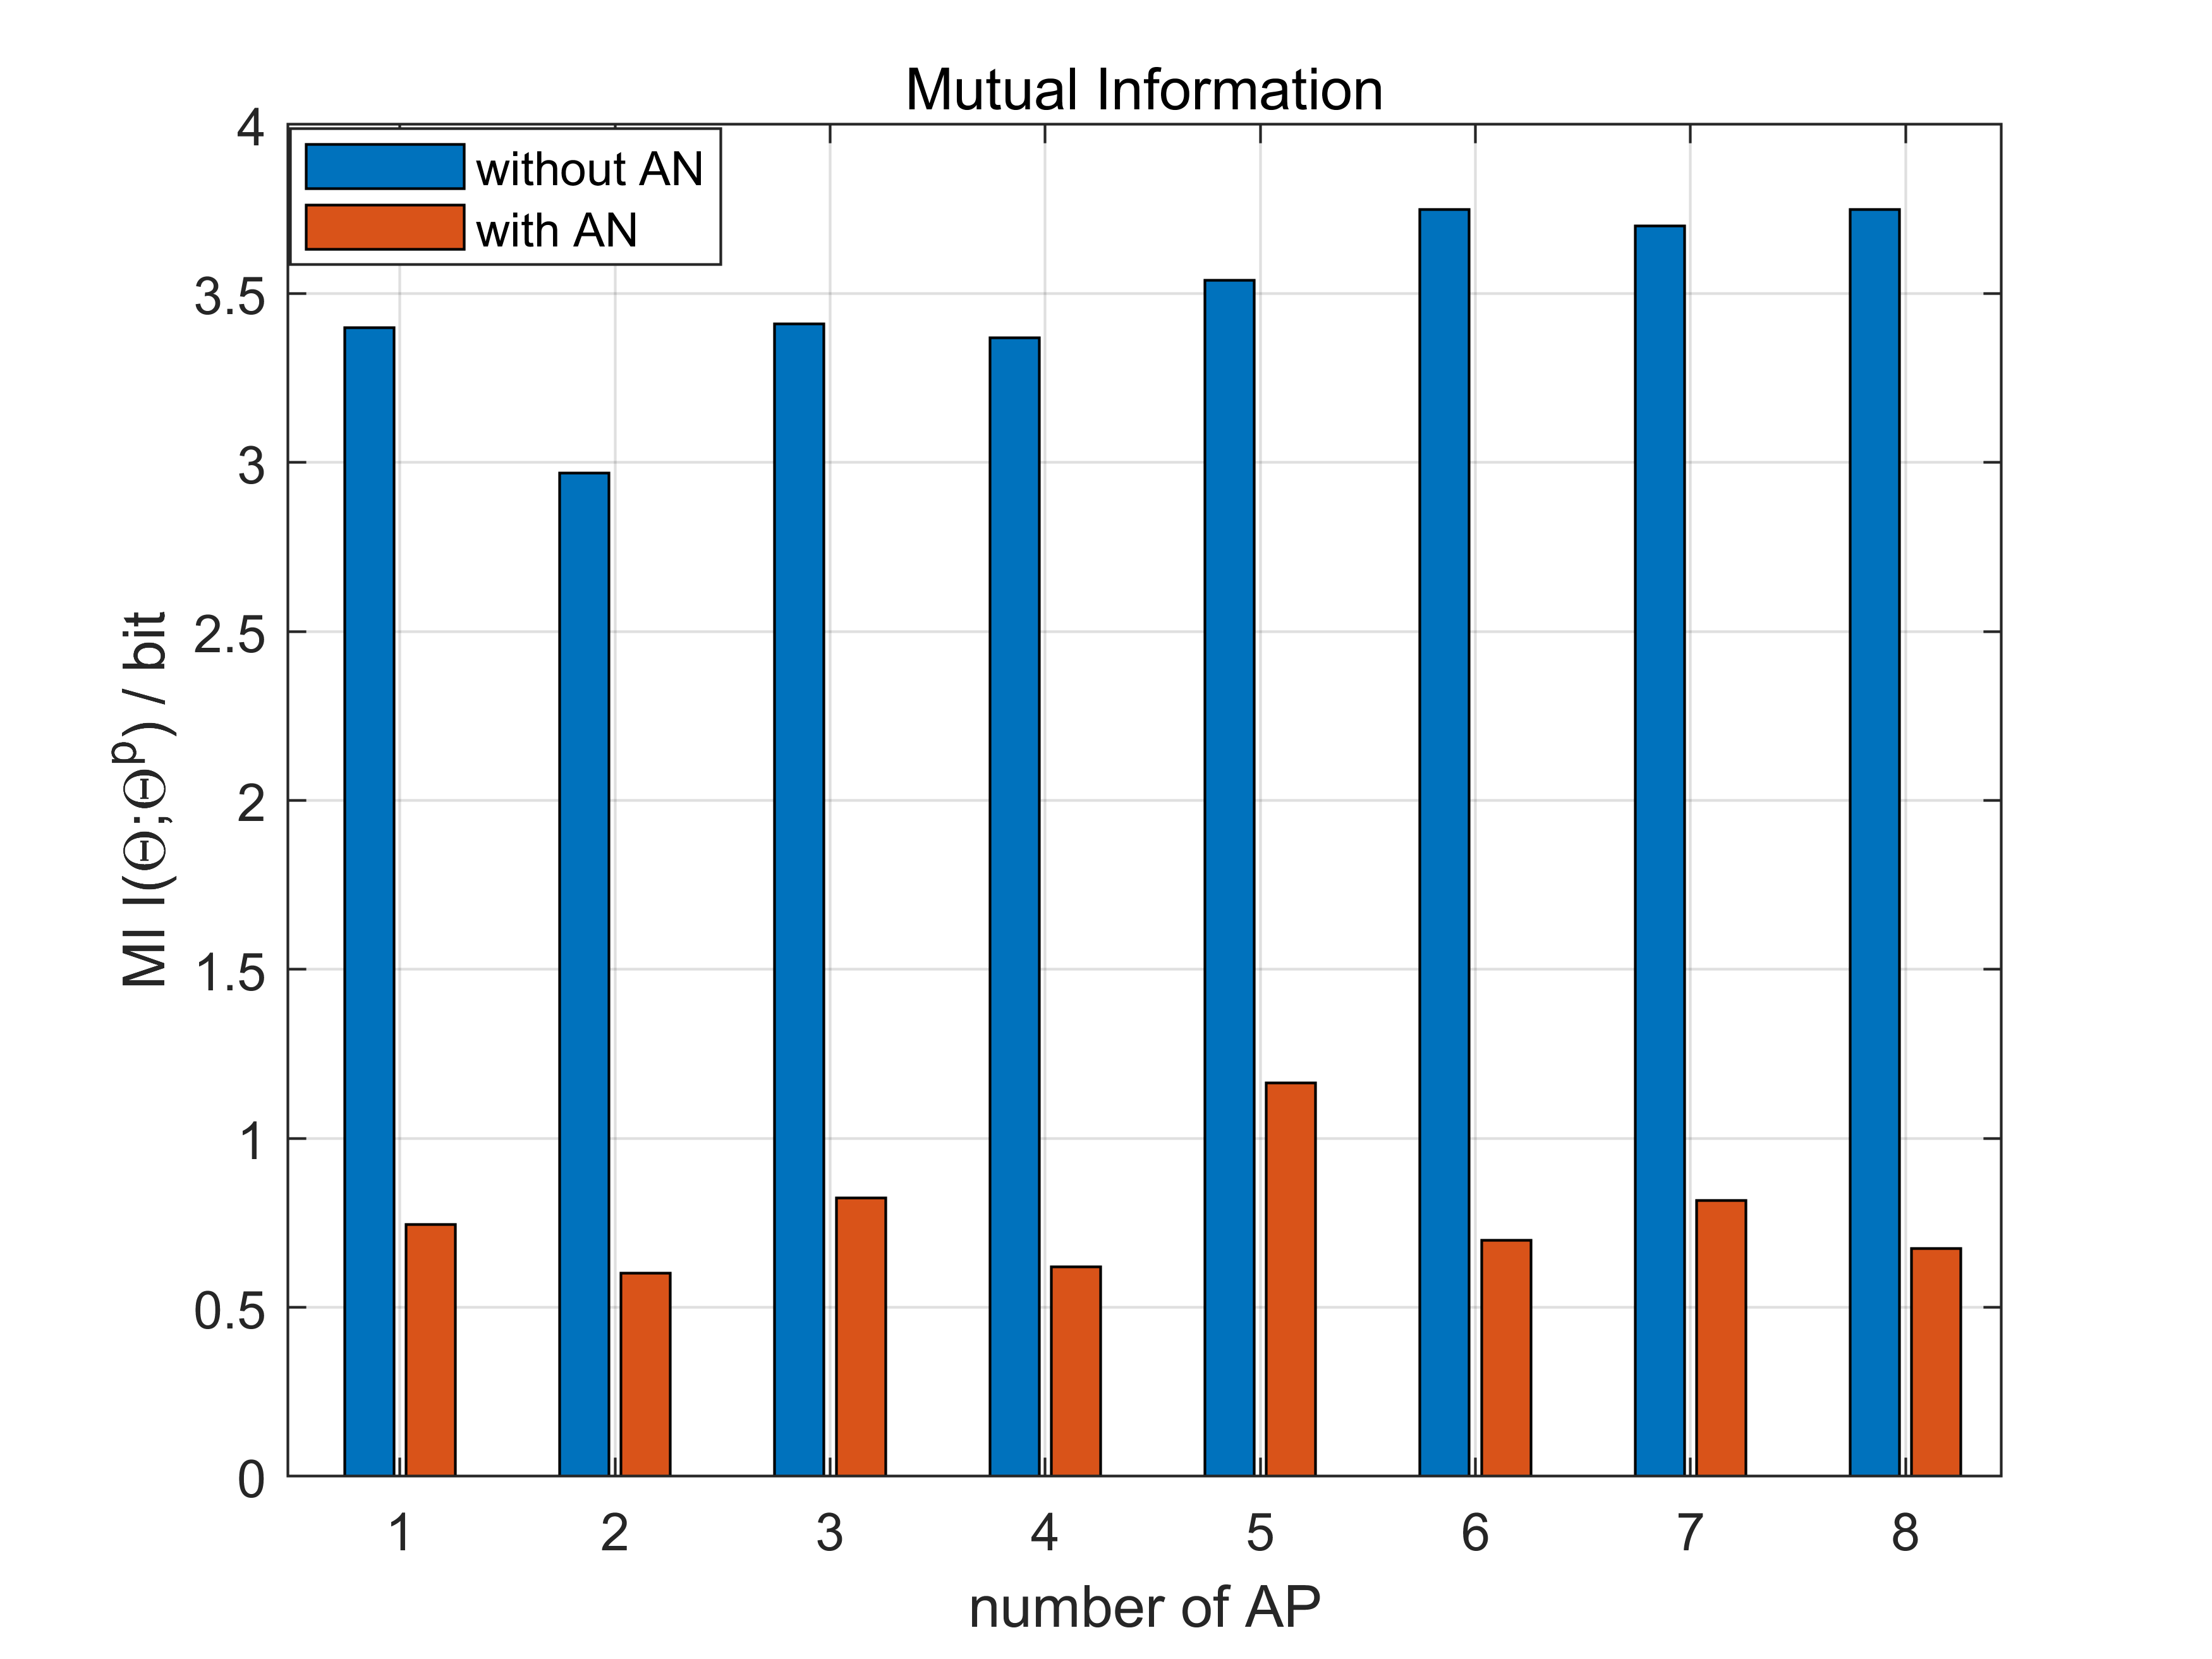
\includegraphics[width=0.98\columnwidth]{MI.png}
    \caption{Directional mutual-information comparison across different APs without and with artificial noise.}
    \label{fig:mi}
\end{figure}

Figure~\ref{fig:mi} shows the mutual-information results for different APs. Without artificial noise, the directional mutual information of the main APs mostly lies in the range of about $3.4$--$4.1$ bit, indicating that the internal adversary can still obtain relatively strong true-direction information from the dominant direction. After artificial noise is introduced, this value drops overall to about $0.8$--$1.1$ bit, showing that the statistical correlation between the true direction and the inferred direction is significantly weakened. This result confirms the effectiveness of the spatial-deception mechanism proposed in Section III from an information-theoretic perspective.

\section{Simulation Results}
For the simulations, the system parameters are as follows: $N_{\mathrm{tx}}=8$ transmitting APs, $N_{\mathrm{rx}}=4$ receiving APs, $N_{\mathrm{UE}}=2$ users, $M_{\mathrm{tx}}=16$ antennas per AP, and $M_{\mathrm{UE}}=16$ antennas per user. The carrier frequency is $1.9$ GHz, the per-AP power budget is $P_T=50$ dBm, the communication threshold is $\Gamma_{\mathrm{comm}}=10$ dB, and both user-side and AP-side noise powers are set to $-94$ dBm. The default target position is $(-75,75)$ m, the users are located at $(50,50)$ m and $(-50,-50)$ m, the receiving APs are placed at $(\pm 150,\pm 150)$ m, and the transmitting APs follow the geometry shown in Fig.~\ref{fig:sim-layout}. For the default target position, the fake-target coordinate is set to $(5,-25)$ m.

\begin{figure}[!t]
    \centering
    \includegraphics[width=0.98\columnwidth]{系统模型分布.jpg}
    \caption{Geometric distribution of the simulation scenario used in Section V, showing the positional relationships among all nodes.}
    \label{fig:sim-layout}
\end{figure}

\begin{figure}[!t]
    \centering
    \begin{subfigure}[t]{0.98\columnwidth}
        \centering
        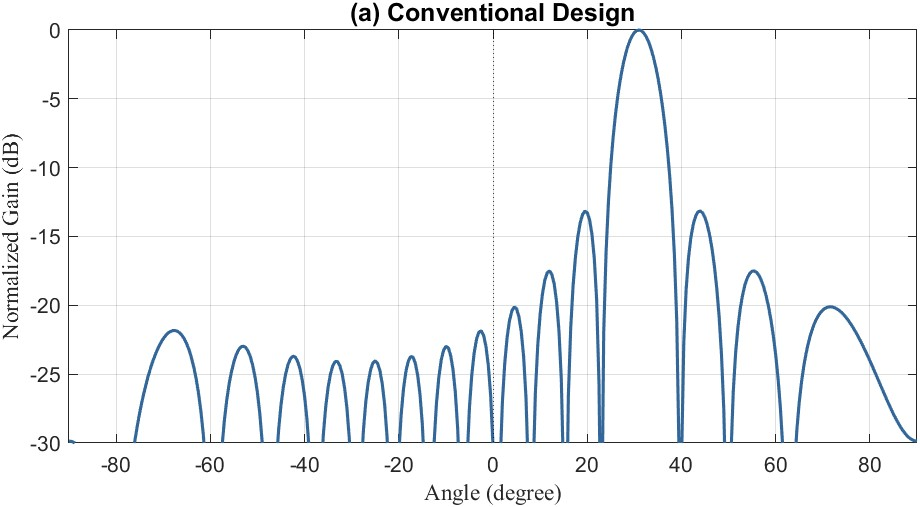
\includegraphics[width=\textwidth]{波束图传统方案.jpg}
        \caption{Conventional JSC design.}
    \end{subfigure}
    \vspace{0.5ex}
    \begin{subfigure}[t]{0.98\columnwidth}
        \centering
        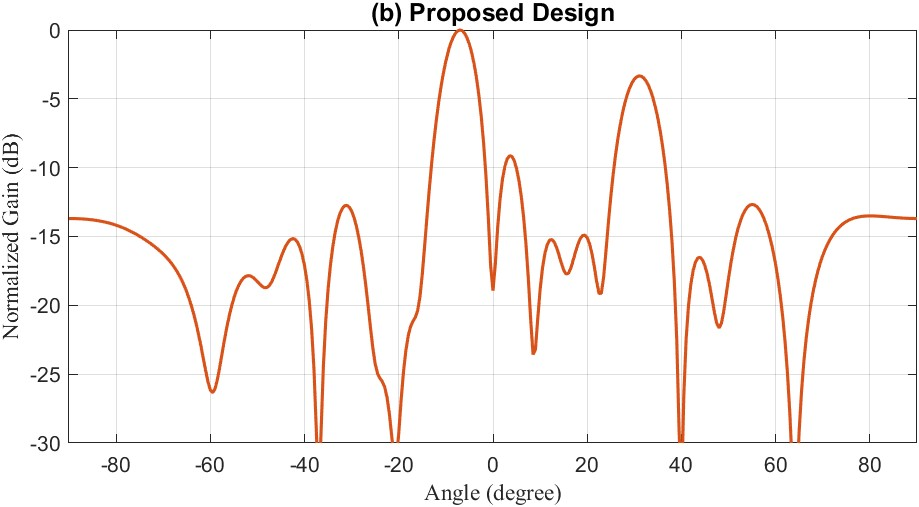
\includegraphics[width=\textwidth]{波束图提出方案.jpg}
        \caption{Proposed AN-aided design.}
    \end{subfigure}
    \caption{Comparison of the normalized transmit beampatterns. The secure design forms an additional misleading peak in the fake direction while preserving a significant response in the true direction.}
    \label{fig:beampatterns}
\end{figure}

Figure~\ref{fig:beampatterns} compares the beampatterns of the conventional design and the proposed design. Without artificial noise, the transmitted energy is mainly concentrated around the true target direction, so the internal adversary can more easily make a judgment from the mainlobe position. After the proposed design is adopted, an additional strong peak appears near the fake direction, and the overall spatial pattern is no longer dominated by a single reliable mainlobe. This phenomenon is the direct manifestation of constraint \eqref{prob:fake} and is also the fundamental reason for the subsequent privacy improvement.

\begin{figure}[t]
    \centering
    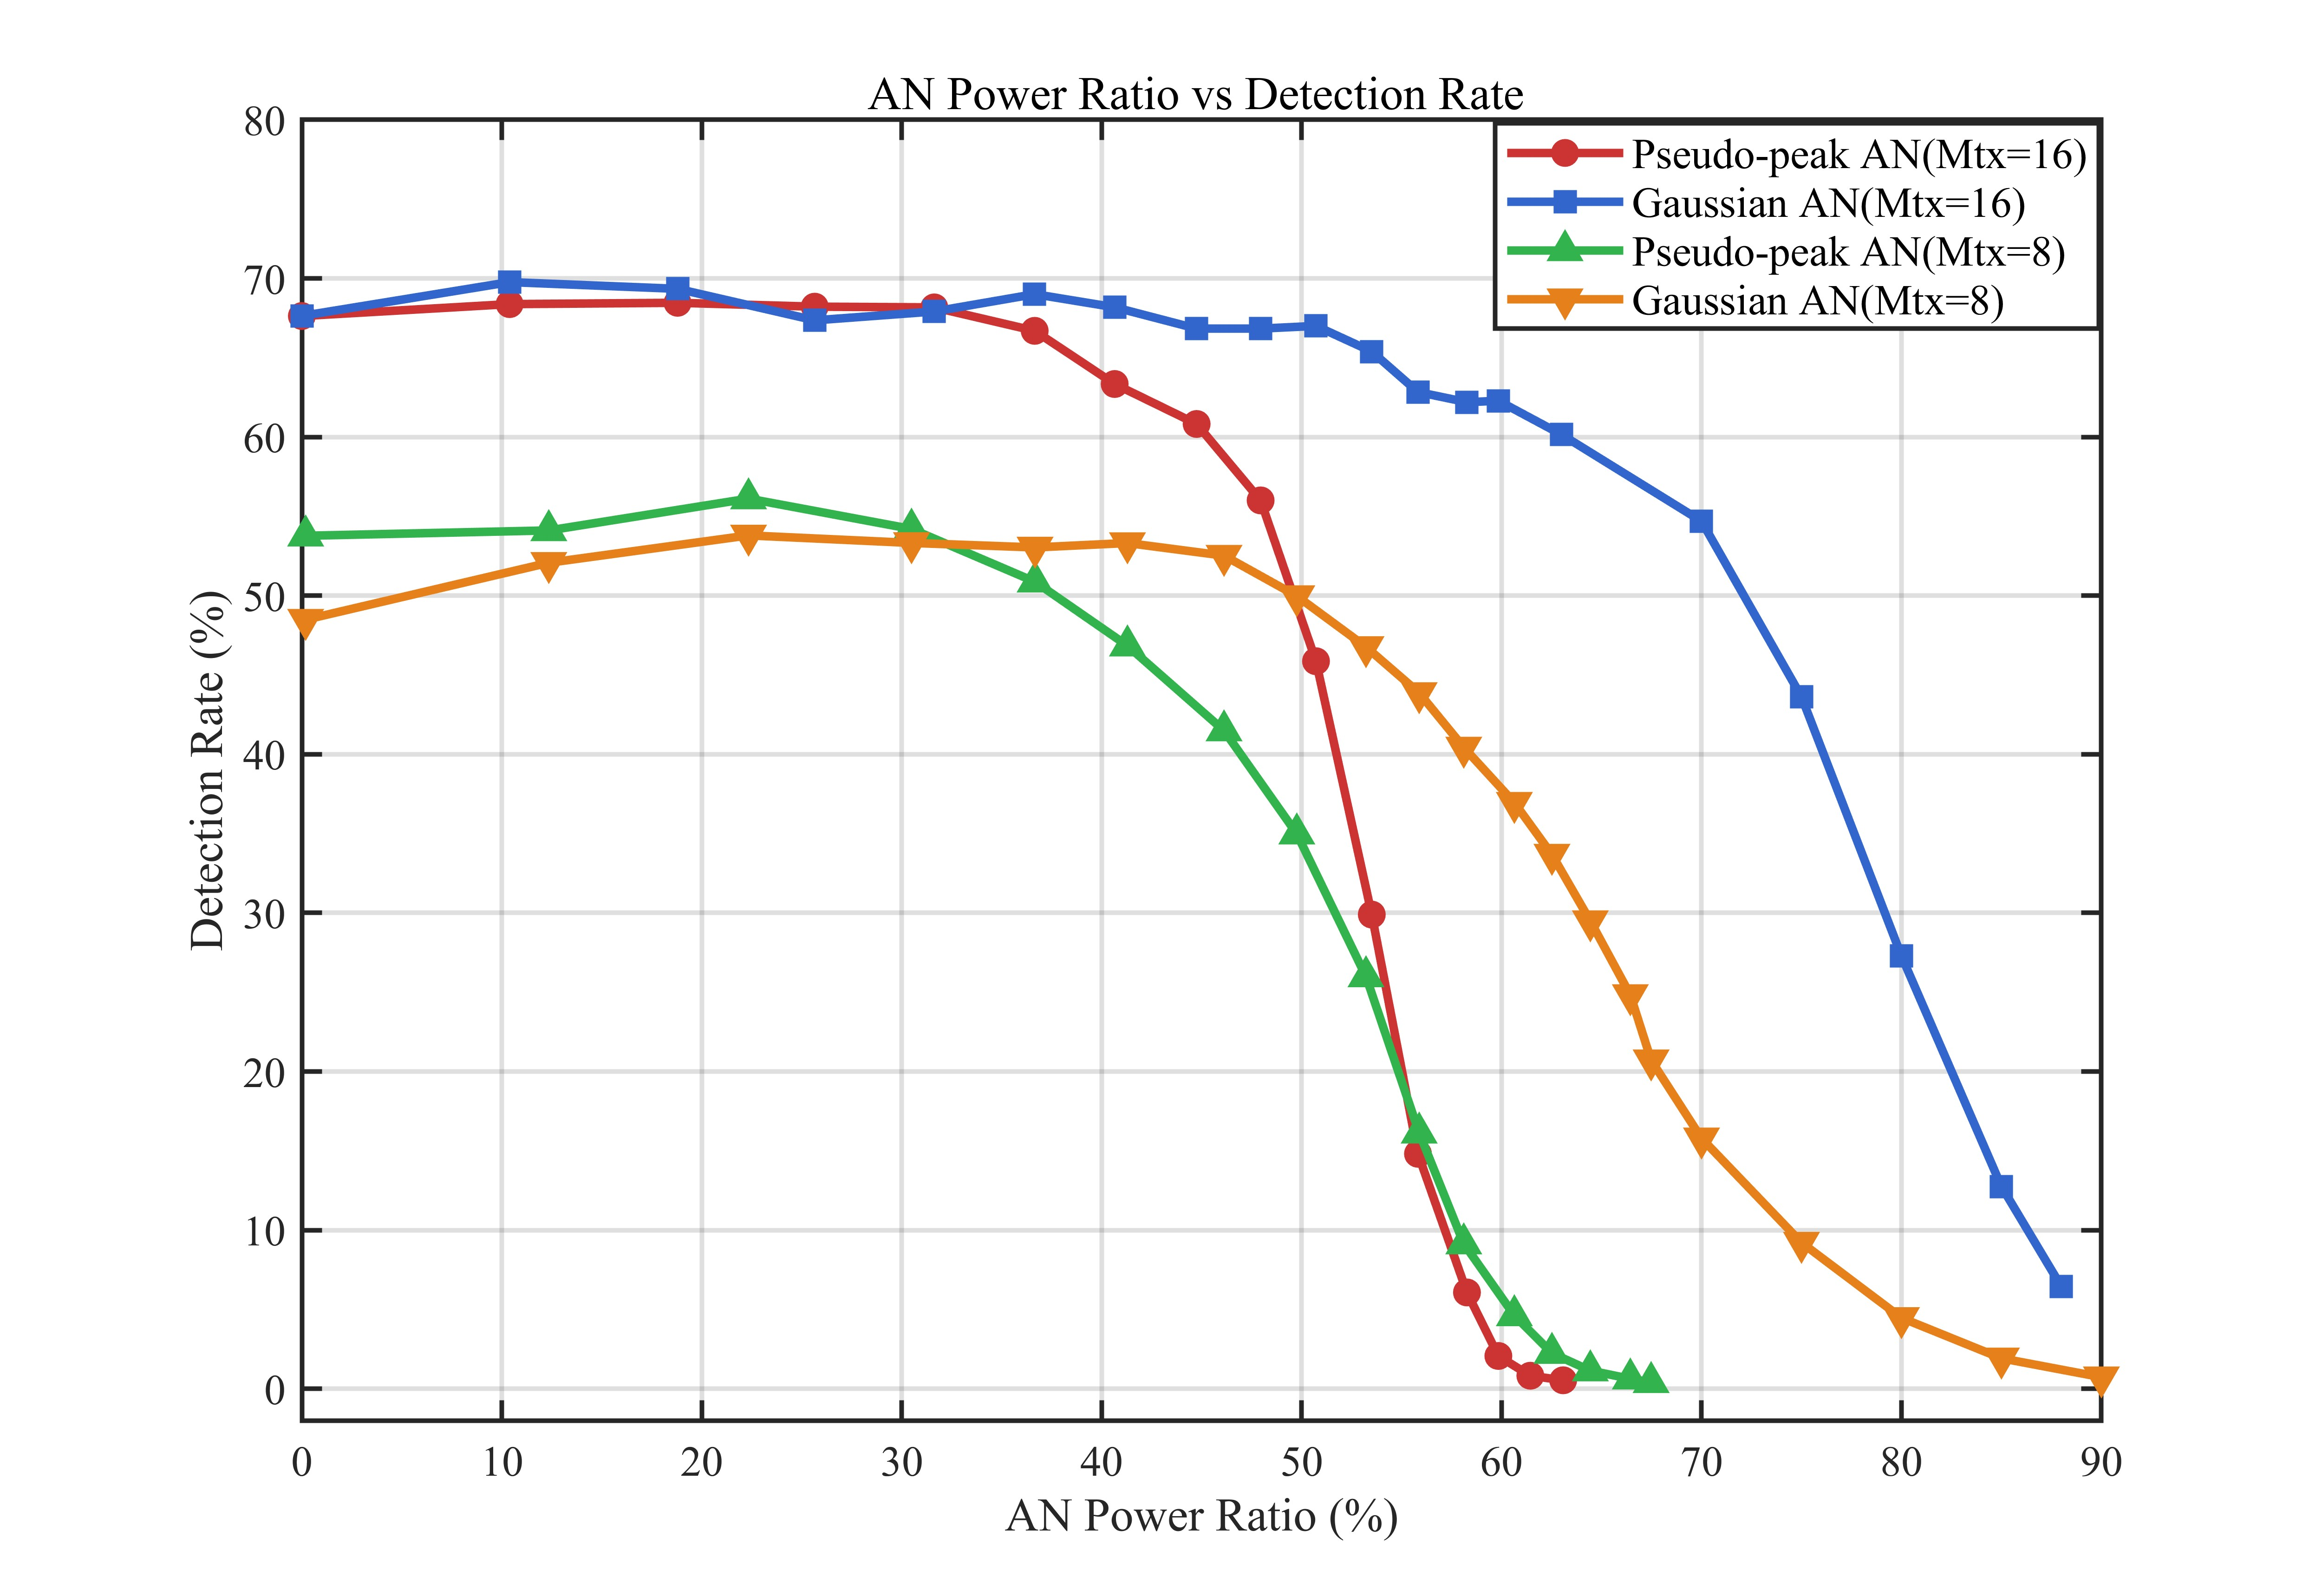
\includegraphics[width=0.98\columnwidth]{guassANvsFakeAN.jpg}
    \caption{Detection-rate comparison between pseudo-peak artificial noise and Gaussian artificial noise.}
    \label{fig:gauss-fake}
\end{figure}

Figure~\ref{fig:gauss-fake} compares the detection-rate curves of pseudo-peak artificial noise and Gaussian artificial noise for different transmit-array sizes. It can be seen that, for both $M_{\mathrm{tx}}=16$ and $M_{\mathrm{tx}}=8$, the pseudo-peak AN curve lies overall to the left of the Gaussian AN curve, which means that the proposed directional pseudo-peak design requires a lower AN-power ratio to achieve the same suppression effect on the detection rate. The reason is that Gaussian artificial noise diffuses almost isotropically inside the null space, so its energy is spread across many irrelevant directions; in contrast, pseudo-peak artificial noise concentrates the available power on the preset fake direction and therefore uses AN power more efficiently in destroying the credibility of the dominant peak.

\begin{figure}[t]
    \centering
    \includegraphics[width=0.98\columnwidth]{diffMue.jpg}
    \caption{Relationship between the AN-power ratio and the internal adversary's detection rate under different numbers of user antennas.}
    \label{fig:diffmue}
\end{figure}

Figure~\ref{fig:diffmue} shows how the AN-power ratio influences the detection rate of the internal adversary under different numbers of user antennas. Overall, all curves decrease continuously as the AN-power ratio increases, which indicates that strengthening artificial noise indeed gradually weakens the internal adversary's capability to judge the true target.

On the one hand, the curves in the transmit-antenna and user-antenna comparisons both follow the overall rule that fewer antennas imply weaker detection capability and a lower detection probability. On the other hand, the ordering of the curves does not remain fixed over the whole AN-power range. For the transmit-antenna comparison, when $M_{\mathrm{tx}}$ decreases, the array aperture becomes smaller, the beam becomes wider, the angular resolution degrades, and the null-space degrees of freedom also shrink. At the same time, the reduction of antenna number lowers the beamforming gain, so under the same AN power the pseudo-peak in the fake direction becomes less prominent. In short, a lower $M_{\mathrm{tx}}$ weakens the deception capability of the generated beampattern. Therefore, when the largest beampattern energy has already become dominated by the pseudo-peak under high AN power, the internal adversary with a lower $M_{\mathrm{tx}}$ may instead exhibit a slightly higher detection rate.

For the user-antenna comparison, a larger $M_{\mathrm{UE}}$ tends to produce a higher detection rate in the low-AN region, because more receive dimensions help the internal adversary execute EM-based beampattern reconstruction and distinguish the true target direction. In the high-AN region, however, a larger $M_{\mathrm{UE}}$ enters the descending regime more rapidly. This is because once the pseudo-peak starts to dominate the beampattern, stronger receive dimensions enable the internal adversary to lock onto the wrong direction more stably, namely, to be misled more accurately. In contrast, when the adversary has fewer antennas, its directional resolution for both the true target and the fake target is weaker, so the curve decays more gradually in the descending region. It is also worth noting that, in the low-AN region, the detection probabilities for $M_{\mathrm{UE}}=16$ and $M_{\mathrm{UE}}=12$ are rather close. This suggests that the influence of antenna number on detection capability has a threshold effect, beyond which further antenna increase has only a limited impact on detection probability. Overall, these phenomena show that the proposed scheme does not merely damage detection by raising the noise floor, but instead changes the adversary's directional-decision mechanism by reshaping the dominant spatial feature.

\begin{figure}[!t]
    \centering
    \begin{subfigure}[t]{0.98\columnwidth}
        \centering
        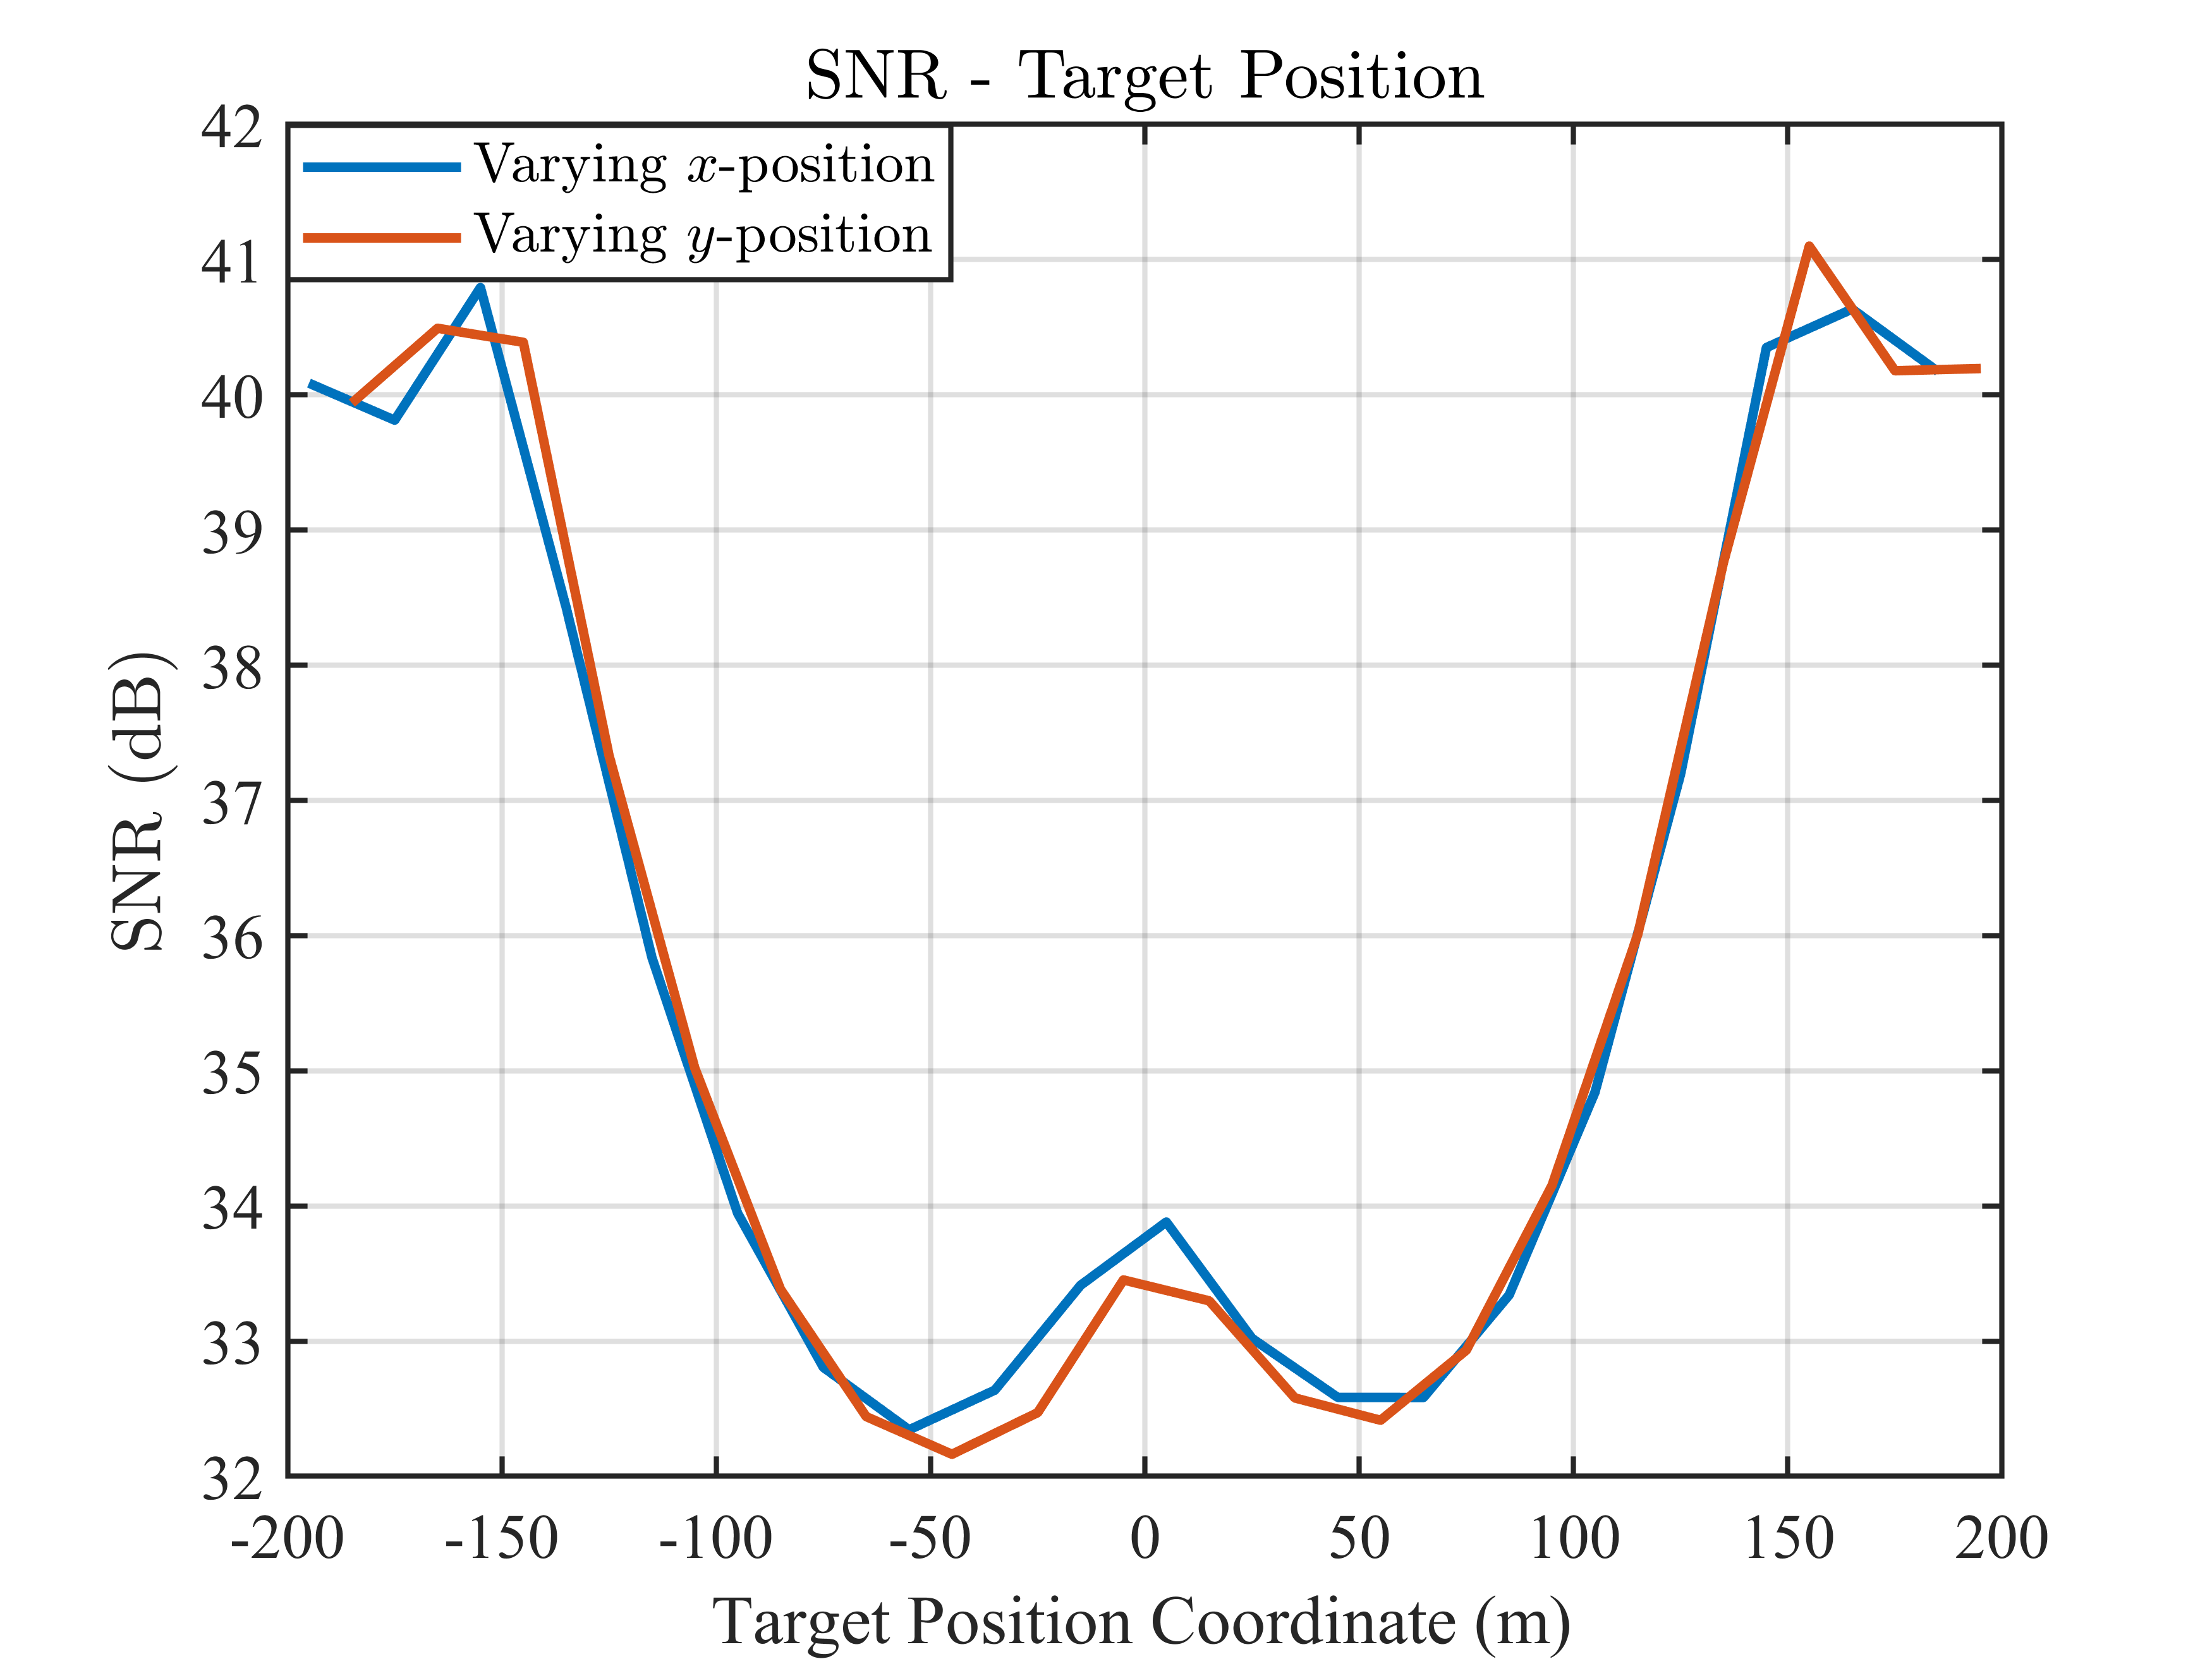
\includegraphics[width=\textwidth]{SNR_vs_Xpos.png}
        \caption{Sensing SNR versus target position.}
        \label{fig:snr-pos}
    \end{subfigure}
    \vspace{0.5ex}
    \begin{subfigure}[t]{0.98\columnwidth}
        \centering
        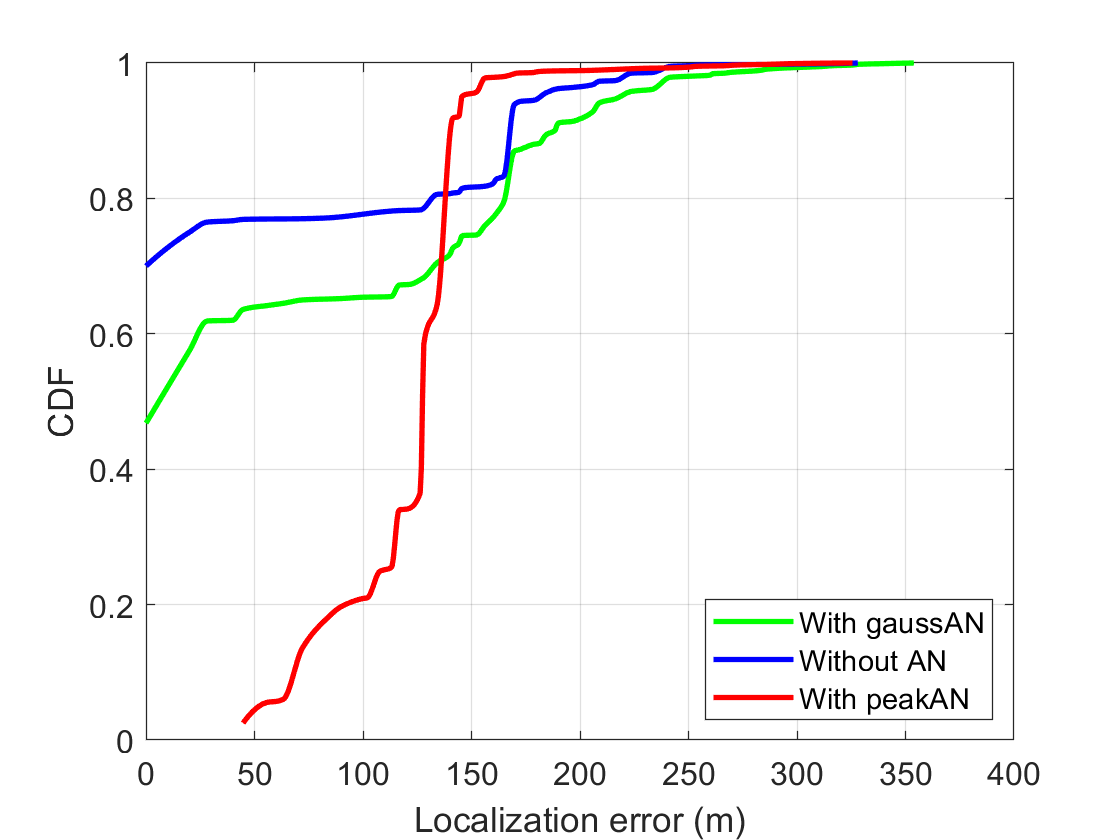
\includegraphics[width=\textwidth]{检测误差CDF.png}
        \caption{CDF of localization error.}
        \label{fig:cdf}
    \end{subfigure}
    \caption{Additional sensing and localization-error results.}
    \label{fig:triple-results}
\end{figure}

Figure~\ref{fig:snr-pos} shows the spatial-geometric dependence of the sensing performance. As the target moves within the prescribed system-model region, the system sensing SNR always remains above about $32$ dB and can reach more than $41$ dB in the edge region. This indicates that the privacy enhancement in this paper is not obtained by damaging the sensing function, but by altering the spatial features seen by the adversary while preserving legitimate sensing capability.

Figure~\ref{fig:cdf} gives the CDF of the localization error of the internal adversary. Under the same power allocation, without artificial noise, many samples correspond to small localization errors, which means that the adversary can often obtain a relatively accurate position estimate. When Gaussian AN is used, the error distribution shifts moderately to the right, but the shift is limited. After the proposed design is adopted, the error distribution shifts significantly toward the larger-distance region, which means that even if the adversary does not fail completely, its estimate is still obviously distorted in terms of spatial position.

\FloatBarrier

\section{Conclusion}
This paper studies sensing-privacy protection against an internal adversary in a multi-static cell-free massive MIMO ISAC system. A potential malicious user in the network can recover transmit spatial features with the help of the EM algorithm and infer the target position from the directional clues provided by multiple transmitting APs. To suppress this leakage process, this paper designs an AN-aided joint beam-optimization method so that the artificial noise forms an observable misleading spatial peak in the fake direction while not affecting the legitimate-user channels. Furthermore, an alternating solution framework based on CCCP and MMSE updates is developed. Simulation results show that the proposed method can significantly reduce the localization capability of the internal adversary while maintaining legitimate sensing performance and substantially lowering its average detection probability. These results indicate that active spatial deception is practically feasible for sensing-privacy protection in cell-free ISAC.


\appendices
\section{Detailed Derivation of the Sensing-SNR Expression}
This appendix gives the detailed derivation of \eqref{eq:snr-sensing}.

For the $r$th receiving AP, after ignoring the receive noise, the effective echo signal can be written as
\begin{equation}
\mathbf{y}_{S,r}[n]=\mathbf{a}(\phi_r)\eta_r[n],
\label{eq:appA-ys-en}
\end{equation}
where
\begin{equation}
\eta_r[n]=\sum_{k=1}^{N_{\mathrm{tx}}}\alpha_{r,k}\sqrt{\beta_{r,k}}\mathbf{a}^H(\phi_k)\mathbf{W}_k\mathbf{s}[n].
\label{eq:appA-eta-en}
\end{equation}
Define the effective row channel
\begin{equation}
\mathbf{H}_{r,\mathrm{eff}}=\sum_{k=1}^{N_{\mathrm{tx}}}\alpha_{r,k}\sqrt{\beta_{r,k}}\mathbf{a}^H(\phi_k)\mathbf{W}_k,
\label{eq:appA-heff-en}
\end{equation}
so that $\eta_r[n]=\mathbf{H}_{r,\mathrm{eff}}\mathbf{s}[n]$.

The desired sensing power at receiver AP $r$ is then
\begin{equation}
P_{S,r}=\mathbb{E}_{\alpha,s}\!\left[\mathbf{y}_{S,r}^H[n]\mathbf{y}_{S,r}[n]\right].
\label{eq:appA-ps1-en}
\end{equation}
Substituting \eqref{eq:appA-ys-en} gives
\begin{align}
P_{S,r}
&=\mathbb{E}_{\alpha,s}\!\left[\eta_r^*[n] \mathbf{a}^H(\phi_r)\mathbf{a}(\phi_r) \eta_r[n]\right] \nonumber\\
&=\mathbf{a}^H(\phi_r)\mathbf{a}(\phi_r)\,\mathbb{E}_{\alpha,s}\!\left[|\eta_r[n]|^2\right].
\label{eq:appA-ps2-en}
\end{align}
Because the steering vector of the $M_{\mathrm{tx}}$-element ULA satisfies
\begin{equation}
\mathbf{a}^H(\phi_r)\mathbf{a}(\phi_r)=M_{\mathrm{tx}},
\label{eq:appA-arraynorm-en}
\end{equation}
we obtain
\begin{equation}
P_{S,r}=M_{\mathrm{tx}}\,\mathbb{E}_{\alpha,s}\!\left[|\eta_r[n]|^2\right].
\label{eq:appA-ps3-en}
\end{equation}

Using $\eta_r[n]=\mathbf{H}_{r,\mathrm{eff}}\mathbf{s}[n]$, the above becomes
\begin{align}
P_{S,r}
&=M_{\mathrm{tx}}\,\mathbb{E}_{\alpha,s}\!\left[\mathbf{s}^H[n]\mathbf{H}_{r,\mathrm{eff}}^H\mathbf{H}_{r,\mathrm{eff}}\mathbf{s}[n]\right] \nonumber\\
&=M_{\mathrm{tx}}\,\mathbb{E}_{\alpha,s}\!\left[\mathrm{Tr}\!\left(\mathbf{H}_{r,\mathrm{eff}}\mathbf{s}[n]\mathbf{s}^H[n]\mathbf{H}_{r,\mathrm{eff}}^H\right)\right].
\label{eq:appA-ps4-en}
\end{align}
Since the communication symbols and sensing symbol are mutually independent and unit-power normalized,
\begin{equation}
\mathbb{E}_{s}\!\left[\mathbf{s}[n]\mathbf{s}^H[n]\right]=\mathbf{I},
\label{eq:appA-ss-en}
\end{equation}
which leads to
\begin{equation}
P_{S,r}=M_{\mathrm{tx}}\,\mathrm{Tr}\!\left(\mathbb{E}_{\alpha}\!\left[\mathbf{H}_{r,\mathrm{eff}}\mathbf{H}_{r,\mathrm{eff}}^H\right]\right).
\label{eq:appA-ps5-en}
\end{equation}

Next, expand the second-order moment. From \eqref{eq:appA-heff-en},
\begin{align}
\mathbf{H}_{r,\mathrm{eff}}\mathbf{H}_{r,\mathrm{eff}}^H
&=\left(\sum_{k=1}^{N_{\mathrm{tx}}}\alpha_{r,k}\sqrt{\beta_{r,k}}\mathbf{a}^H(\phi_k)\mathbf{W}_k\right)
\left(\sum_{j=1}^{N_{\mathrm{tx}}}\alpha_{r,j}\sqrt{\beta_{r,j}}\mathbf{a}^H(\phi_j)\mathbf{W}_j\right)^H \nonumber\\
&=\sum_{k=1}^{N_{\mathrm{tx}}}\sum_{j=1}^{N_{\mathrm{tx}}}\alpha_{r,k}\alpha_{r,j}^*\sqrt{\beta_{r,k}\beta_{r,j}}\left(\mathbf{a}^H(\phi_k)\mathbf{W}_k\right)\left(\mathbf{a}^H(\phi_j)\mathbf{W}_j\right)^H.
\label{eq:appA-expand-en}
\end{align}
Assuming independent scattering coefficients for different Tx-Rx pairs,
\begin{equation}
\mathbb{E}\!\left[\alpha_{r,k}\alpha_{r,j}^*\right]=
\begin{cases}
\sigma_{r,k}^2, & k=j,\\
0, & k\neq j.
\end{cases}
\label{eq:appA-rcs-en}
\end{equation}
Hence all cross terms vanish after expectation and we obtain
\begin{equation}
\mathbb{E}_{\alpha}\!\left[\mathbf{H}_{r,\mathrm{eff}}\mathbf{H}_{r,\mathrm{eff}}^H\right]
=\sum_{k=1}^{N_{\mathrm{tx}}}\sigma_{r,k}^2\beta_{r,k}\left(\mathbf{a}^H(\phi_k)\mathbf{W}_k\right)\left(\mathbf{a}^H(\phi_k)\mathbf{W}_k\right)^H.
\label{eq:appA-expheff-en}
\end{equation}
The trace of each scalar term equals its Frobenius norm squared, so
\begin{equation}
\mathrm{Tr}\!\left(\mathbb{E}_{\alpha}\!\left[\mathbf{H}_{r,\mathrm{eff}}\mathbf{H}_{r,\mathrm{eff}}^H\right]\right)
=\sum_{k=1}^{N_{\mathrm{tx}}}\sigma_{r,k}^2\beta_{r,k}\left\|\mathbf{a}^H(\phi_k)\mathbf{W}_k\right\|_F^2.
\label{eq:appA-trace-en}
\end{equation}
Substituting \eqref{eq:appA-trace-en} into \eqref{eq:appA-ps5-en} gives
\begin{equation}
P_{S,r}=M_{\mathrm{tx}}\sum_{k=1}^{N_{\mathrm{tx}}}\sigma_{r,k}^2\beta_{r,k}\left\|\mathbf{a}^H(\phi_k)\mathbf{W}_k\right\|_F^2.
\label{eq:appA-ps-final-en}
\end{equation}

For the receiver noise $\mathbf{n}_r[n]\sim\mathcal{CN}(\mathbf{0},\sigma_n^2\mathbf{I})$, the average noise power is
\begin{equation}
P_{N,r}=\mathbb{E}\!\left[\mathbf{n}_r^H[n]\mathbf{n}_r[n]\right]=M_{\mathrm{tx}}\sigma_n^2.
\label{eq:appA-pn-en}
\end{equation}
Summing the signal and noise powers across all receiver APs yields
\begin{align}
\gamma_t
&=\frac{\sum_{r=1}^{N_{\mathrm{rx}}}P_{S,r}}{\sum_{r=1}^{N_{\mathrm{rx}}}P_{N,r}} \nonumber\\
&=\frac{\sum_{r=1}^{N_{\mathrm{rx}}}\sum_{k=1}^{N_{\mathrm{tx}}}\sigma_{r,k}^2\beta_{r,k}\left\|\mathbf{a}^H(\phi_k)\mathbf{W}_k\right\|_F^2}{N_{\mathrm{rx}}\sigma_n^2} \nonumber\\
&=\sum_{k=1}^{N_{\mathrm{tx}}}\left(\frac{\sum_{r=1}^{N_{\mathrm{rx}}}\sigma_{r,k}^2\beta_{r,k}}{N_{\mathrm{rx}}\sigma_n^2}\right)\left\|\mathbf{a}^H(\phi_k)\mathbf{W}_k\right\|_F^2,
\label{eq:appA-gamma-en}
\end{align}
which is exactly \eqref{eq:snr-sensing} and \eqref{eq:ck}.

\section{Supplementary Derivations for the CCCP Convexification}
This appendix corresponds to Section III-B in the main text. The detailed derivations of the first-order lower bounds are given here to explain the origins of \eqref{eq:obj-lb}, \eqref{eq:signal-lb}, and \eqref{eq:fake-lb}.

\subsection{First-Order Lower-Bound Formula for Complex Variables}
For a complex vector variable $\mathbf{v}$ and its perturbation $\Delta\mathbf{v}$, the first-order expansion can be written as
\begin{equation}
f(\mathbf{v}+\Delta\mathbf{v})
=
f(\mathbf{v})
+2\Re\!\left\{\left(\frac{\partial f}{\partial \mathbf{v}^*}(\mathbf{v})\right)^H\Delta\mathbf{v}\right\}
+o(\|\Delta\mathbf{v}\|).
\label{eq:appB-complex-taylor-en}
\end{equation}
For a matrix variable $\mathbf{W}$, the corresponding first-order expansion is
\begin{equation}
f(\mathbf{W}+\Delta\mathbf{W})
=
f(\mathbf{W})
+2\Re\!\left\{\mathrm{Tr}\!\left[\left(\frac{\partial f}{\partial \mathbf{W}^*}(\mathbf{W})\right)^H\Delta\mathbf{W}\right]\right\}
+o(\|\Delta\mathbf{W}\|_F).
\label{eq:appB-matrix-taylor-en}
\end{equation}
For any Hermitian matrix $\mathbf{A}\succeq 0$ and a complex variable $\mathbf{x}$, the function
\begin{equation}
f(\mathbf{x})=\mathbf{x}^H\mathbf{A}\mathbf{x}
\end{equation}
is convex. Moreover,
\begin{equation}
\frac{\partial f}{\partial \mathbf{x}^*}(\mathbf{x}) = \mathbf{A}\mathbf{x}
\end{equation}
Likewise, for a complex matrix variable $\mathbf{W}$, the function $f(\mathbf{W})=\mathrm{Tr}(\mathbf{W}^H\mathbf{A}\mathbf{W})$ satisfies
\begin{equation}
\frac{\partial f}{\partial \mathbf{W}^*}(\mathbf{W}) = \mathbf{A}\mathbf{W}
\end{equation}
Therefore, at the iterate $\mathbf{x}^{(v)}$, the first-order Taylor expansion gives the global lower bound
\begin{equation}
f(\mathbf{x})\ge f\big(\mathbf{x}^{(v)}\big)+2\Re\!\left\{\left(\mathbf{A}\mathbf{x}^{(v)}\right)^H\big(\mathbf{x}-\mathbf{x}^{(v)}\big)\right\}.
\label{eq:appB-taylor-en}
\end{equation}
Equivalently,
\begin{equation}
\mathbf{x}^H\mathbf{A}\mathbf{x}\ge 2\Re\!\left\{\left(\mathbf{A}\mathbf{x}^{(v)}\right)^H\mathbf{x}\right\}-\left(\mathbf{x}^{(v)}\right)^H\mathbf{A}\mathbf{x}^{(v)}.
\label{eq:appB-basiclb-en}
\end{equation}
This formula will be used to linearize the objective function, the useful-signal numerator, and the fake-direction artificial-noise term, respectively.

\subsection{Derivation of the Objective Surrogate}
For AP $k$, the objective contribution in Section III-B is
\begin{equation}
f_{0,k}(\mathbf{W}_k)=\mathrm{Tr}(\mathbf{W}_k^H\mathbf{A}_k\mathbf{W}_k).
\end{equation}
At the iterate $\mathbf{W}_k^{(v)}$, \eqref{eq:appB-basiclb-en} gives
\begin{align}
f_{0,k}(\mathbf{W}_k)
&\ge 2\Re\!\left\{\mathrm{Tr}\!\left[(\mathbf{A}_k\mathbf{W}_k^{(v)})^H\mathbf{W}_k\right]\right\}
-\mathrm{Tr}\!\left[(\mathbf{W}_k^{(v)})^H\mathbf{A}_k\mathbf{W}_k^{(v)}\right].
\label{eq:appB-objlb-en}
\end{align}
Using $\mathrm{Tr}(\mathbf{W}_k^H\mathbf{A}_k\mathbf{W}_k)=\|\mathbf{a}^H(\phi_k)\mathbf{W}_k\|_F^2$, the same lower bound can also be written as
\begin{align}
f_{0,k}(\mathbf{W}_k)
&\ge 2\Re\!\left\{\mathbf{a}^H(\phi_k)\mathbf{W}_k\mathbf{W}_k^{(v)H}\mathbf{a}(\phi_k)\right\} \nonumber\\
-\|\mathbf{a}^H(\phi_k)\mathbf{W}_k^{(v)}\|_F^2.
\label{eq:appB-objlb-alt-en}
\end{align}
Equation \eqref{eq:obj-lb} in the main text is exactly the affine lower bound generated by this step, and substituting it into \eqref{eq:tx-orig-obj} yields the surrogate objective \eqref{eq:ftilde}.

\subsection{Derivation of the SINR Surrogate}
For the desired-signal numerator in \eqref{eq:tx-orig-sinr}, define $s_i^{(v)}=s_i(\mathbf{W}^{(v)})$ with $s_i(\mathbf{W})$ given by \eqref{eq:si-def}. Applying \eqref{eq:appB-basiclb-en} to $|s_i(\mathbf{W})|^2$ yields
\begin{equation}
|s_i(\mathbf{W})|^2\ge 2\Re\!\left\{\left(s_i^{(v)}\right)^*s_i(\mathbf{W})\right\}-|s_i^{(v)}|^2.
\label{eq:appB-signal-lb-en}
\end{equation}
Using this lower bound inside \eqref{eq:tx-orig-sinr} produces the affine approximation \eqref{eq:stilde} and the convex constraint \eqref{eq:tx-cvx-sinr} in the main text.

\subsection{Derivation of the Fake-Direction Surrogate}
For the fake-direction term in \eqref{eq:tx-orig-fake}, applying \eqref{eq:appB-basiclb-en} at the iterate $\mathbf{z}_k^{(v)}$ gives
\begin{equation}
\mathbf{z}_k^H\mathbf{A}_{\mathrm{f},k}\mathbf{z}_k
\ge 2\Re\!\left\{\left(\mathbf{A}_{\mathrm{f},k}\mathbf{z}_k^{(v)}\right)^H\mathbf{z}_k\right\}-\left(\mathbf{z}_k^{(v)}\right)^H\mathbf{A}_{\mathrm{f},k}\mathbf{z}_k^{(v)}.
\label{eq:appB-zlb-en}
\end{equation}
Using $\mathbf{z}_k^H\mathbf{A}_{\mathrm{f},k}\mathbf{z}_k=\|\mathbf{a}^H(\phi_{\mathrm{fake},k})\mathbf{z}_k\|^2$, the same lower bound can also be written as
\begin{align}
\|\mathbf{a}^H(\phi_{\mathrm{fake},k})\mathbf{z}_k\|^2
&\ge 2\Re\!\left\{\mathbf{a}^H(\phi_{\mathrm{fake},k})\mathbf{z}_k\mathbf{z}_k^{(v)H}\mathbf{a}(\phi_{\mathrm{fake},k})\right\} \nonumber\\
-\|\mathbf{a}^H(\phi_{\mathrm{fake},k})\mathbf{z}_k^{(v)}\|^2.
\label{eq:appB-zlb-alt-en}
\end{align}
Substituting this lower bound into \eqref{eq:tx-orig-fake} yields the affine surrogate \eqref{eq:ztilde} and the convexified constraint \eqref{eq:tx-cvx-fake}. Together with \eqref{eq:obj-lb} and \eqref{eq:signal-lb}, these steps recover the main-text convex program \eqref{eq:tx-cvx}.

\bibliographystyle{IEEEtran}
\bibliography{references}

\end{document}
